
% documentclass options:
% ngerman is needed for hyphenation if the thesis contains parts written in German
% BCOR is binding correction
% if you'd rather have a one sided thesis, add `onside' to the documentclass
\documentclass[11pt, a4paper, BCOR=10mm, english, ngerman]{scrbook}

% include all packages and define commands in setup.tex

%------------------------------------------------------------------------------
%       package includes
%------------------------------------------------------------------------------
    % font encoding is set up for pdflatex, for other environments see
    % http://tex.stackexchange.com/questions/44694/fontenc-vs-inputenc
    \usepackage[T1]{fontenc}  % 8-bit fonts, improves handling of hyphenations
    \usepackage[utf8x]{inputenc}
    % provides `old' commands for table of contents. Eases the ability to switch
    % between book and scrbook
    \usepackage{scrhack}
    \usepackage{caption}
    \usepackage{subcaption}
    \usepackage{multirow}
    \usepackage{listings}

    % ------------------- layout, default -------------------
    % adjust the style of float's captions, separated from text to improve readabilty
    \usepackage[labelfont=bf, labelsep=colon, format=hang, textfont=singlespacing]{caption}
    \usepackage{chngcntr}  % continuous numbering of figures/tables over chapters
    \counterwithout{equation}{chapter}
    \counterwithout{figure}{chapter}
    \counterwithout{table}{chapter}

    % Uncomment the following line if you switch from scrbook to book
    % and comment the setkomafont line
    %\usepackage{titlesec}  % remove "Chapter" from the chapter title
    %\titleformat{\chapter}[hang]{\bfseries\huge}{\thechapter}{2pc}{\huge}
    \setkomafont{chapter}{\normalfont\bfseries\huge}

    \usepackage{setspace}  % Line spacing
    \onehalfspacing
    % \doublespacing  % uncomment for double spacing, e.g. for annotations in correction

    % ------------------- functional, default-------------------
    \usepackage[dvipsnames]{xcolor}  % more colors
    \usepackage{array}  % custom format per column in table - needed on the title page
    \usepackage{graphicx}  % include graphics
    \usepackage{amsmath}  % |
    \usepackage{amsthm}   % | math, bmatrix etc
    \usepackage{amsfonts} % |
    \usepackage{calc}  % calculate within LaTeX
    \usepackage[unicode=true,bookmarks=true,bookmarksnumbered=true,
                bookmarksopen=true,bookmarksopenlevel=1,breaklinks=false,
                pdfborder={0 0 0},backref=false,colorlinks=false]{hyperref}


    %==========================================
    % You might not need the following packages, I only included them as they
    % are needed for the example floats
    % ------------------- functional, custom -------------------
    \usepackage{algorithm,algpseudocode}
    \usepackage{bm}  % bold greek variables (boldmath)
    \usepackage{tikz}
    \usetikzlibrary{positioning}  % use: above left of, etc

    % Improves general appearance of the text
    \usepackage[protrusion=true,expansion=true, kerning]{microtype}

%------------------------------------------------------------------------------
%       (re)new commands / settings
%------------------------------------------------------------------------------
    % ----------------- referencing ----------------
    \newcommand{\secref}[1]{Section~\ref{#1}}
    \newcommand{\chapref}[1]{Chapter~\ref{#1}}
    \renewcommand{\eqref}[1]{Equation~(\ref{#1})}
    \newcommand{\figref}[1]{Figure~\ref{#1}}
    \newcommand{\tabref}[1]{Table~\ref{#1}}

    % ------------------- colors -------------------
    \definecolor{darkgreen}{rgb}{0.0, 0.5, 0.0}
    % Colors of the Albert Ludwigs University as in
    % https://www.zuv.uni-freiburg.de/service/cd/cd-manual/farbwelt
    \definecolor{UniBlue}{RGB}{0, 74, 153}
    \definecolor{UniRed}{RGB}{193, 0, 42}
    \definecolor{UniGrey}{RGB}{154, 155, 156}


    % ------------------- layout -------------------
    % prevents floating objects from being placed ahead of their section
    \let\mySection\section\renewcommand{\section}{\suppressfloats[t]\mySection}
    \let\mySubSection\subsection\renewcommand{\subsection}{\suppressfloats[t]\mySubSection}


    % ------------------- marker commands -------------------
    % ToDo command
    \newcommand{\todo}[1]{\textbf{\textcolor{red}{(TODO: #1)}}}
    \newcommand{\extend}[1]{\textbf{\textcolor{darkgreen}{(EXTEND: #1)}}}
    % Lighter color to note down quick drafts
    \newcommand{\draft}[1]{\textbf{\textcolor{NavyBlue}{(DRAFT: #1)}}}


    % ------------------- math formatting commands -------------------
    % define vectors to be bold instead of using an arrow
    \renewcommand{\vec}[1]{\mathbf{#1}}
    \newcommand{\mat}[1]{\mathbf{#1}}
    % tag equation with name
    \newcommand{\eqname}[1]{\tag*{#1}}


    % ------------------- pdf settings -------------------
    % ADAPT THIS
    \hypersetup{pdftitle={The great title!},
                pdfauthor={FirstName LastName},
                pdfsubject={Undergraduate thesis at the Albert Ludwig University of Freiburg},
                pdfkeywords={deep learning, awesome algorithm,  undergraduate thesis},
                pdfpagelayout=OneColumn, pdfnewwindow=true, pdfstartview=XYZ, plainpages=false}


    %==========================================
    % You might not need the following commands, I only included them as they
    % are needed for the example floats

    % ------------------- Tikz styles -------------------
    \tikzset{>=latex}  % arrow style


    % ------------------- algorithm ---------------------
    % Command to align comments in algorithm
    \newcommand{\alignedComment}[1]{\Comment{\parbox[t]{.35\linewidth}{#1}}}
    % define a foreach command in algorithms
    \algnewcommand\algorithmicforeach{\textbf{foreach}}
    \algdef{S}[FOR]{ForEach}[1]{\algorithmicforeach\ #1\ \algorithmicdo}


\begin{document}
    \pagestyle{empty} % no header and no page number
    % disable hyper links to remove warning "destination with same identifier"
    % this means within this section nothing can be referenced with a hyperlink
    \hypersetup{pageanchor=false}
        \newcommand\T{\rule{0pt}{2.6ex}}       % Top strut
    \newcommand\B{\rule[-1.2ex]{0pt}{0pt}} % Bottom strut

    
\begin{titlepage}
\begin{center}

\newcommand{\HorizontalLine}{\rule{\linewidth}{0.3mm}}

{\Large Master's Thesis}\\[1.3cm]


% _____________________________________________________________________________
\HorizontalLine \\[0.4cm]
\begin{spacing}{3}
    {\huge \bfseries Design and Implementation of a } \\
    {\huge \bfseries Configurable Preferential Web Search Engine} \\
\end{spacing}
\HorizontalLine \\[1.5cm]
% _____________________________________________________________________________


{\Huge Alhajras Algdairy} \\[2cm]


\begin{tabular}[hc]{>{\huge}l >{\huge}l}
  Examiner: & Prof. Dr. Hannah Bast \\[0.3cm]
  Advisers: & Natalie Prange \\[1.2cm]
\end{tabular}
\vfill  % move the following text to the bottom

\Large {
    Albert-Ludwigs-University Freiburg\\
    Faculty of Engineering\\
    Department of Computer Science\\
    Chair of Algorithms and Data Structures\\[1cm]

    October 31\textsuperscript{st}, 2023\\
}
\end{center}
\end{titlepage}

% title page back
\ \vfill \ \\  % at least one space required before vfill
\
\textbf{Writing period}            \smallskip{} \\
08.\,05.\,2023 -- 31.\,10.\,2023   \bigskip{} \\
\
\textbf{Examiner}                  \smallskip{} \\
Prof. Dr. Hannah Bast               \bigskip{} \\
\
\textbf{Advisers}                  \smallskip{} \\
Natalie Prange

    \pagestyle{plain} % remove chapter name from top, page number at the bottom
    \frontmatter  % roman page numbers
    % official declaration from the examination office; to be sure double
% check the wording on their website
% (https://www.tf.uni-freiburg.de/studies/exams/thesis/thesis_formatting.html#erklaerung)

\chapter*{Declaration}

I hereby declare, that I am the sole author and composer of my thesis and that no other sources or learning aids, other than those listed, have been used. Furthermore, I declare that I have acknowledged the work of others by providing detailed references of said work.  \newline
I hereby also declare, that my Thesis has not been prepared for another examination
or assignment, either wholly or excerpts thereof.
\\[3\normalbaselineskip]
\begin{tabular}{p{\textwidth/2} l}
  \rule{\textwidth/3}{0.4pt}   &   \rule{\textwidth/3}{0.4pt} \\
  Place, Date                  &   Signature
\end{tabular}

    \chapter*{Abstract}
In this thesis, I introduce Scriburg, a prototype for a large-scale search engine that can be configured to suit specific user preferences. Scriburg has been developed to crawl efficiently and index web content, offering a range of settings through a user-friendly interface. The system is designed to handle small and large websites, making it adaptable to various scenarios. Scriburg is particularly well-suited for situations where users have a specific interest in a subset of the web, such as a particular domain or a select group of web pages. In today's business landscape, online content analysis plays a crucial role in making informed decisions. However, existing solutions in this space are often proprietary, needing more transparency in their code and flexibility for customization and scalability. Despite the significance of web search engines, there remains a need for further academic research focused on developing and designing open-source search engine solutions that can be readily used and extended by a wide range of users.
    \tableofcontents
    \listoffigures
    \listoftables
    \listofalgorithms
    \hypersetup{pageanchor=true}  % re-enable hyperlinking

    \mainmatter  % Arabic page numbers
    \chapter{Introduction}
\label{chap:introduction}
\section{Motivation}

The World Wide Web (WWW) contains an enormous amount of data; this data is increasing each day rapidly. The amount of total data created and replicated is expected to grow to more than 180 zettabytes by 2025 according to Statista. The growth is expected to continue as more smartphones are more and more affordable, and more people can reach the internet. Moreover, due to the COVID-19 pandemic, more companies started offering work remotely, more shops created online stores, and more services switched to cloud-based. This change in society during the last few years has made the internet a vital part of our day-to-day life.   

Although the data is available, making a helpful meaning is a challenge. Search engines, for example, try to organize and index that information to make them easily searchable by the end user. Furthermore, collecting data can help spot competitors and have a deeper meaning in the market. Additionally, data scientists are now playing essential roles in most organizations and enterprises to understand consumer needs by collecting and analyzing data from the web.  


Although some websites provide APIs to provide organized information about their services, for example, some airline companies provide API that serves information about their flight schedules, other online shops also provide a documented API to get helpful information about their available products. This is not a guaranteed approach to gathering data, as not all websites offer an excellent documented API. For example, social media websites are reluctant to give information about their users, which is understandable. What if you would like to go through all comments and classify them as spam or not? Depending only on the assumption of having an API for each website is a fragile approach. 

Information retrieval (IR) is a term introduced in 1951 by Calvin
Mooers. It is accessing and retrieving data from a vast pool of unstructured information. The generic use case of the IR is to 

Amount of data created, consumed, and stored 2010-2020, with forecasts to 2025
Published by 
Petroc Taylor
, Sep 8, 2022
https://www.statista.com/statistics/871513/worldwide-data-created/#:~:text=The%20total%20amount%20of%20data,to%20more%20than%20180%20zettabytes.
\section{Contributions}
\section{Chapter Overview}

    \chapter{Related Work}
\label{chap:relatedwork}
\numberwithin{equation}{chapter}
Creating a generic configurable search engine that includes a simple user interface will require research on how the current search engine works and what are the existing commercial or open-source solutions that offer a similar feature that allows the search engine to be configured via user interface reactions. This chapter will explain an overview of the Google search engine architecture since the basic architecture concepts will be reused with some modifications in this thesis. Then a list of the existing solutions used to crawl the web will be discussed.  



\section{High Level Google Architecture}

The Google search engine's design gives a good overview of the essential components to create a scalable search engine. Hence, it is a great starting point for any search engine research; we will explain it in this section. Most code written in the Google search engine was implemented in C or C++ for efficiency and because it can run on either Solaris or Linux [2]. Google uses distributed crawlers to download internet web pages. The URLserver keeps a list of the available found URLs that need to be crawled by the crawlers. URLserver acts as a load balancer that sends the URLs to the following free crawler. Afterwards, the crawlers download the documents needed from the page, associate a unique ID for this page called docID, and then the page's content are stored in Soreservers. Storeservers then compress the pages and save them on a repository. The indexer component then uncompresses the pages and parses them. Each document is then converted into a set of words called hits. The hits represent the word and its position in the document. Afterwards, the indexer distributes those hits into barrels. Moreover, the indexer collects links found in the crawled page and stores them in the anchor's file. The anchors' file contains the links and their relationship with each other [2].


\begin{figure}[h]	
     \centering
     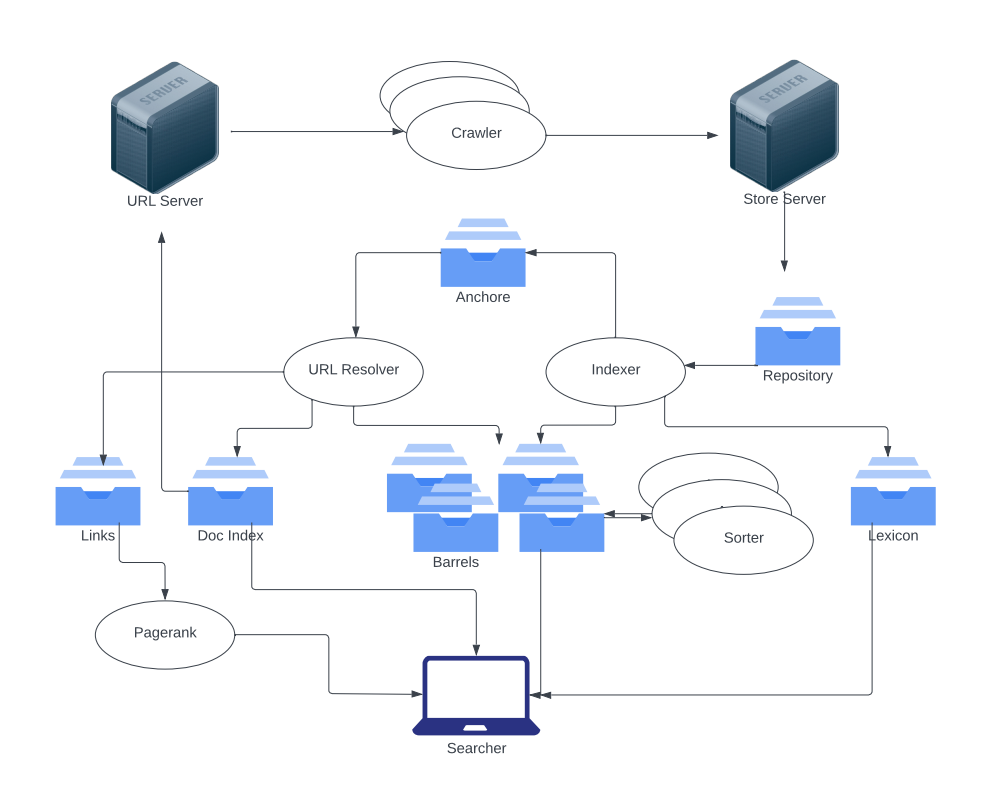
\includegraphics[width=10cm]{images/google_arch.png}
     \caption{High level view of Google web crawlers archeticture.}
     \label{fig:google-arch}
\end{figure}

The URLresolver reads the links from the anchors' file and converts the relative URLs into absolute URLs. The URLs are then assigned to their docID. The links database saves pairs of docIDs that will be used to compute PageRanks for all the documents. 

Initially organized by docID, the barrels are then rearranged by the sorter based on wordID. This process generates an inverted index. Moreover, the sorter generates a list of wordIDs and corresponding offsets within the inverted index. 

\section{Web Crawlers}
The concept of web crawling dates back to the early 1990s when the World Wide Web was still in its infancy.

WebCrawler, created by Brian Pinkerton in 1994, is considered the first true web crawler-powered search engine. While some may claim that title for Wandex is due to its potential, it was never designed to be used in this way. Wandex lacked some critical features to make it a general-purpose search engine.

One of the major innovations of WebCrawler was its full-text searchability. This ability made it popular and highly functional. It continues to operate as a search engine, although not as popular as Google, Yahoo, Bing, Yandex, or Baidu.

Modern web crawlers face many challenges and complexities, such as dynamic content, user interaction, authentication, robots.txt files, and ethical issues. Some examples of modern web crawlers are Googlebot, Bingbot, and Internet Archive

Web crawlers have evolved during the last few decades, with different designs and implementations to crawl and index the internet. Below is an enumeration of some of the architectural designs utilized in the development of all-encompassing web crawlers [3]:


\begin{itemize}
  \item \textbf{RBSE [Eic94]} Considered as one of the first Web crawlers to be published. Made of two components: the first component,
“spider”, uses a queue in a database. The second component, “mite”, is a modified browser that downloads the pages from the Web.
  \item \textbf{WebCrawler [Pin94]}  The initial publicly accessible full-text index of a specific portion of the World Wide Web was established. The approach involved leveraging lib-WWW for page downloads and employing an additional tool to parse and arrange URLs, ensuring a breadth-first approach to navigating the web graph.
  \item \textbf{World Wide Web Worm [McB94]} was a crawler designed to construct a basic index comprising document titles and corresponding URLs. This index could be queried by utilising the grep command in the UNIX operating system.
  \item \textbf{Google Crawler [BP98]} Google has been the market's dominant search engine for the last few decades. In March 2023, Google’s global market share was 85.53% [4].
The crawler was integrated with the indexing, and since this thesis has some similarity with the Google search engine design, we will explain this in-depth in the ext subsection [Google architecture]
  \item \textbf{Ubicrawler [BCSV04]} Is a Java-based distributed crawler with no central process and several identical “agents”. The crawler is implemented to provide high scalability and be tolerant of failures.
\end{itemize}

Although the previously mentioned crawlers offer a wide range of features and are great to be used as generic crawlers to fetch all web pages, they need to provide a simple user interface to configure them based on user needs. This is what this thesis tries to tackle and investigate. 

Nowadays, data scientist uses different tools to crawl and parse internet content. Each tool has its pros and cons and serves a different use case than the other. The following list goes through some of the most well know crawlers and explains how the proposed solution in this thesis differs.  


\begin{itemize}
  \item \textbf{Beautiful Soup:} Beautiful Soup is an open-source library that stands out as a widely used web scraping library that simplifies retrieving data from HTML and XML documents. Beautiful Soup demonstrates exceptional proficiency in parsing HTML documents, streamlining the task of retrieving particular components like headings, paragraphs, tables, and links. Beautiful Soup is not a search engine. It lacks the most fundamental search engine components; hence, it requires programming skills and can only be used to implement a search engine. Beautiful Soup can only parse the first seen page HTML version. Meaning it does not include the Javascript code. This is bad as most modern web pages use Javascript heavily to improve the page's latency. For example, pagination will be an issue for Beautiful Soup.

  \item \textbf{Scrapy:} It is an open-source, powerful and flexible tool that easily crawls and parses different websites. It allows the creation of custom spiders to crawl multiple pages. Easy to scale makes it suitable for large projects. This tool is perfect for programmers but not for non-technical users, as it requires good knowledge of Python programming.

  \item \textbf{Selenium:} It is an open-source, robust and adaptable solution for web scraping, enabling the automation of browser actions, interaction with web pages, and data extraction from online sources. It shares some features with the Beautiful Soupe as it is an excellent tool for parsing the HTML DOM. Still, it also overcomes the issue previously mentioned about rendering Javascript and supporting dynamic contents as paginations. Interactive browser automation makes it easy to mimic the user's behaviour which makes it easier to navigate towards hidden content that requires events and human interactions. Selenium alone can be used as a search engine; however, it will be used in this thesis as a fundamental tool for the search engine implemented.    

  \item \textbf{ParseHub:} A web crawler tool with a friendly User Interface requiring no programming skills. It is one of the top choices of most data scientists. The massive advantage of ParseHub is the point-and-click interface provided. It makes data extraction extremely easy. ParseHub offers both free and paid plans. The free plan allows users to scrape up to 200 pages per run, which, as we will see, is too slow for a crawler. Moreover, it is not possible to configure the crawling algorithms with this tool, and the indexing component does not exist. Since this tool is the most similar tool to the solution implemented by this thesis, it will be used as a comparison in the evaluation chapter. 
\end{itemize}

    \chapter{Background}\
\label{chap:background}
This section tackles the fundamental principles and groundwork of the theory encompassing concepts, terminology, and methodologies related to search engines as applied within this thesis. Section \ref{sec:web-search-engine} dives into the essential components and characteristics required to implement the search engine discussed in this thesis. Section \ref{sec:crawler} provides a comprehensive examination of the crawler's specifications and architecture. Section \ref{sec:indexing} offers an in-depth explanation of the fundamental indexing terms and concepts essential to this thesis, while Section \ref{sec:ranking} explores the ranking score used in this research.


\section{Web Search Engine}
\label{sec:web-search-engine}
Web Search Engine is software that collects information from the web and indexes them efficiently to optimize the searching process by the end user. When users enter their queries to ask for information, the engine performs queries, looks up the pre-built organized index, and returns relevant results. Search Engine Results Pages, known as SERPs, present the returned results. The result is then ranked based on predefined criteria. 

Web search engines use web crawlers or spiders to collect and harvest the internet, jumping from one page to another. Each page can contain several links. The crawler's task is to find the links, visit them, and harvest them. Followed by crawlers, indexing is the next process where information is organized and optimized for search.

\begin{figure}[h]	
     \centering
         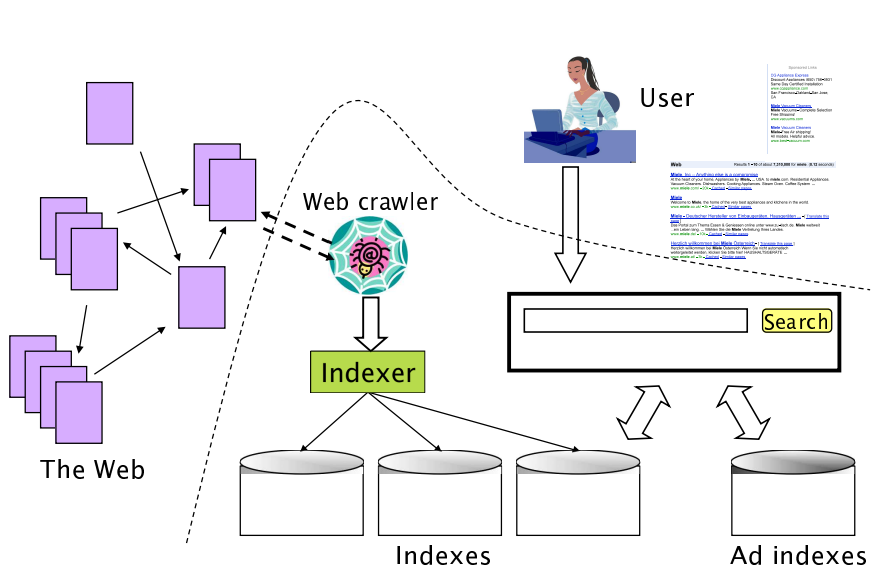
\includegraphics[width=10cm]{images/engine_components.png}
              \caption{An overview of a generic search engine system.}
     \label{fig:search-engine-overvoew}
\end{figure}

\subsection{Requierments and Features}
Regardless of their implementation and design, all search engines share certain features and prerequisites crucial for their effectiveness. Below is a compilation of the most essential features: 

\begin{itemize}
	\item[] \textbf{Web Crawling and Indexing:} As shown in Figure \ref{fig:search-engine-overvoew}, the initial step in the search engine's operation is web crawling. Crawlers initiate the process by connecting to the web and downloading the required pages. Subsequently, indexing comes into play, where the downloaded files are organized and indexed to enhance querying and search efficiency. Parsing the downloaded pages can be carried out in either the crawling phase or during indexing, and Scriburg, this parsing occurs during the crawling process. It is worth noting that, in Scriburg, pages are not downloaded; the targeted documents are parsed, stored in the database, and the pages themselves are discarded.
  \item[] \textbf{Ranking and Relevancy:} As indicated in Figure \ref{fig:search-engine-overview}, when users input a query to search for relevant documents, they face the Search Engine Results Pages (SERP). Users typically focus on the top results while overlooking the lower results. Hence, we must maintain relevancy. Ensuring relevance is a challenging task. Ranking the discovered documents and prioritizing the most pertinent documents at the top and the less relevant ones further down is crucial. 
  \item[] \textbf{Scalability and Performance:} A distributed system is essential for managing the extensive data and traffic demands. A load balancer is critical in distributing the crawling tasks efficiently among nodes and threads. In this, we will discuss the implemented loading balance mechanism to distribute the crawling tasks among the crawlers. 

\end{itemize}

\section{Cralwer}
\label{sec:crawler}
Web crawler or spider is a software which gathers pages information from the web, to prived the necessary data to the Indexer to build a search engine. The essential role of crawlers is to effectively and reliably collect as much information from the web as possible. This thesis invests more time on this component than the Indexer as it serves as the bottleneck to the Search engine performance. There are different types and categories of crawlers. The first category is  \textbf{Universal or Broad crawler}. This category of web crawlers does not confine itself to webpages of a specific topic or domain; instead, they continuously traverse links without limitations, collecting all encountered webpages. Google and Bing use this type of crawler. The second category is called \textbf{Preferential crawler (Focused crawler)}. Focused crawlers target specific topics, themes, or domains \cite{wires}. They are designed to gather information from a particular domain or subject area, providing specialized search results. In this thesis, a Focused crawler has been implemented and used. 

\subsection{Cralwer Specifications}
\label{sec:cralwer-specifications}
Crawlers can display a diverse range of features and specifications. Nevertheless, certain essential elements must be incorporated, while others are critical for ensuring a reliable and functional crawler. Further details can be explored in the book referenced as \cite{introduction-ir}.

\begin{itemize}
\item[] \textbf{Robustness:} Web crawlers can be fragile and easy to break due to the nature of the dynamic contents on the web and the internet connection. Crawlers may encounter broken links, leading to errors and incomplete indexing. Some websites may block or ban crawlers' IP addresses if they perceive them as causing too much traffic or disruption. Web crawlers must identify those edge cases and obstacles and tackle them.

\item[] \textbf{Politeness:} The crawler implementation can be unintentionally dangerous if incorrectly designed. A Denial of service DoS and a Distributed Denial of service DDoS attacks can occur due to an irresponsible crawler implementation. Hence, crawlers must respect website policies and avoid breaking up web services and loading the servers.

\item[] \textbf{Performance and Efficiency:} The crawling system should use various resources, such as processing power, storage capacity, and network bandwidth. Moreover, the crawler should be able to function in distributed microservices across multiple machines.

\item[] \textbf{Freshness:} Obtaining recent versions of previously accessed pages, ensuring the search index remains updated.
\end{itemize}

\subsection{Crawler Architecture}

The simple crawler architecture includes the following fundamental modules, as shown in the following Figure \ref{fig:web-crawler-arch
}. The Fetch module communicates with the internet and collects the pages passed by the URL Frontier module using HTTP requests from the URLs. The URL frontier module contains a list of the URLs that need to be fetched by the Fetch module. Parsing module that takes the page content found by the Fetch module and parses the page content to find the next links to be passed to the URL frontier and also to parse any value needed from the page, like text and images. The following step involves screening the parsed document to eliminate previously visited URLs, duplicate content, and pages that are prohibited by the website. The Domain Name System (DNS)\footnote{The Domain Name System (DNS) is a distributed naming system for internet resources, linking information to domain names.} resolution module identifies the web server from which to retrieve the page indicated by a given URL \cite{introduction-ir}. The DNS will be excluded in this thesis and will not be discussed. 

\begin{figure}[h]	
     \centering
     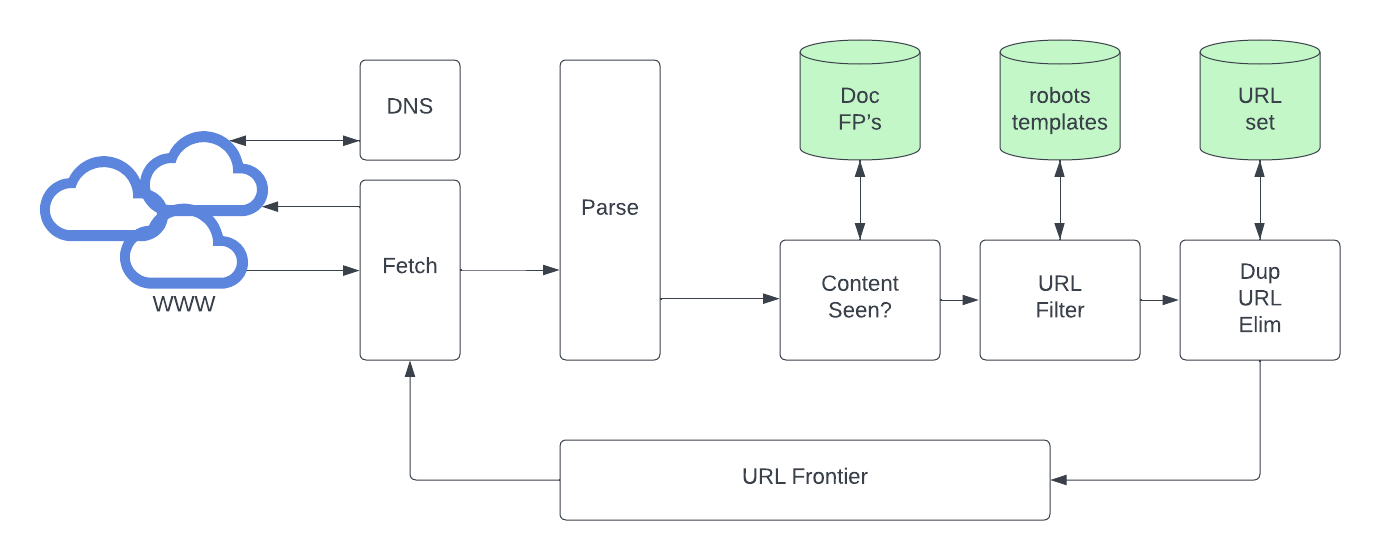
\includegraphics[width=10cm]{images/crawler_architecture.png}
     \caption{A generic web crawler architecture overview \cite{introduction-ir}.}
     \label{fig:web-crawler-arch}
\end{figure}

The crawling process begins with adding a seed URL to the URL frontier as a starting point. The crawler retrieves and stores the corresponding page for parsing. The page's textual content, embedded links, and images are extracted during parsing, with the content prepared for use by the search engine's indexer. Each parsed link undergoes filtering to determine if it is eligible for inclusion in the URL frontier.

Following parsing, a filtering process is essential. Firstly, the content's uniqueness is verified using a fingerprint, often a checksum stored in Doc FP's database. Next, newly parsed URLs are filtered based on various criteria, such as excluding URLs outside the target country or restricted URLs. Domain administrators can specify additional filtering rules, often outlined in a Robots.txt\footnote{More information about Robots.txt can be found in the following link:  \url{https://en.wikipedia.org/wiki/Robots.txt}} file. The Robots Exclusion Protocol (Robots.txt) file is a widely recognized standard websites use to communicate which parts of the site are accessible to web crawlers and other web robots.

The Robots.txt file can be obtained at the start of the crawling process and cached for efficiency, assuming it will not change during crawling. This approach is more efficient than making repeated HTTP requests for the file, reducing the number of requests and server load. Including Robots.txt in the crawling process aligns with the politeness guidelines discussed in the crawler specifications section \ref{sec:cralwer-specifications}.

\subsection{Crawler Data Structure}
Scriburg employs two distinct data structures for its crawling implementation: it utilizes Breadth First Search (BFS) and Depth First Search (DFS).

\textbf{Breadth First Search (BFS):} Considering the link planned for crawling as a vertex, it is worth noting that web pages can be conceptualized as graphs rather than trees. In contrast to trees, graphs can include cycles, which means we might revisit the same vertex. For instance, a basic illustration of this is the home page link, which essentially represents a self-loop in a graph. We can maintain two distinct data structures to prevent processing a vertex multiple times: "Visited" and "Not Visited" vertices. The "Visited" vertices can be stored in a hashmap where the link serves as the key, and the boolean value represents whether the link has already been visited (true for visited, false for unvisited). The second data structure is a queue containing links that still need to be visited.

\begin{figure}[ht] 
  \begin{subfigure}[b]{0.5\textwidth}
    \centering
    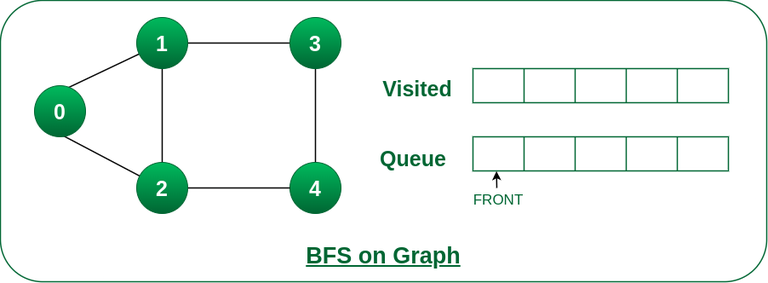
\includegraphics[width=0.75\textwidth]{images/bfs-1.png} 
    \caption{Initial condition} 
    \label{fig7:a} 
    \vspace{4ex}
  \end{subfigure}%% 
  \begin{subfigure}[b]{0.5\textwidth}
    \centering
    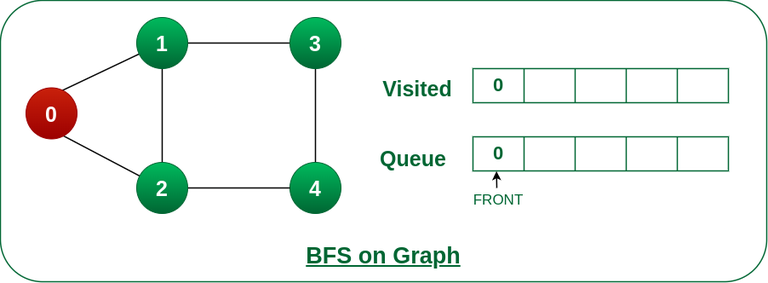
\includegraphics[width=0.75\textwidth]{images/bfs-2.png} 
    \caption{Visit the 0 vertex}  
    \label{fig7:b} 
    \vspace{4ex}
  \end{subfigure} 
  \begin{subfigure}[b]{0.5\textwidth}
    \centering
    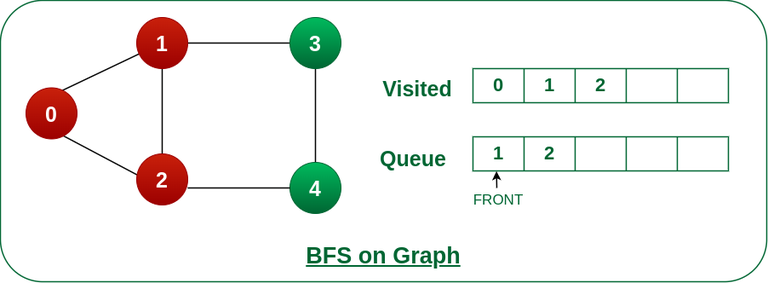
\includegraphics[width=0.75\textwidth]{images/bfs-3.png} 
    \caption{Visit 1 and 2 vertices} 
    \label{fig7:c} 
  \end{subfigure}%%
  \begin{subfigure}[b]{0.5\textwidth}
    \centering
    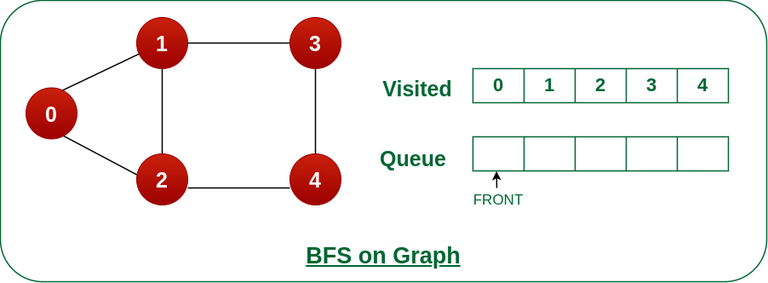
\includegraphics[width=0.75\textwidth]{images/bfs-4.png} 
    \caption{Completed condition} 
    \label{fig7:d} 
  \end{subfigure} 
  \caption{Illustration of the Breadth First Search or BFS for a Graph algorithm.
 \cite{bfs}}
  \label{fig:bfs} 
\end{figure}

The traversal proceeds from the root by visiting all the nodes within a specific level before moving on to the next level. This is accomplished by employing a queue. The unvisited nodes adjacent to the current level are enqueued, while the nodes in the current level are marked as visited and dequeued. One way to perceive this is by initiating the crawling process from the seed URL page, which serves as the root node, and the next level represents all the links discovered within the root page.

Figure \ref{fig:bfs} illustrates the BFS algorithm in operation to enhance visual understanding. Let us visualize a seed URL, denoted as vertex 0. The seed URL page contains two additional links, 1 and 2. The page represented by vertex 1 contains three links: 0, 2, and 3. Similarly, the page associated with vertex 2 includes three links: 0, 1, and 4. Our primary aim is to visit all nodes (links), which is the fundamental objective of the crawler. The crawler must avoid infinite looping and avoid revisiting previously visited nodes (links).

Initially, the queue and the visited hashmap are empty of any entries, which is the ideal state of the crawler. As the crawler launches on its crawling journey, it begins by pushing the seed URL, identified as node 0, into the queue and setting it as visited after visiting it. Subsequently, once the 0 page has been visited, it is dequeued, and the following two discovered links, 1 and 2, are added to the queue. These links, 1 and 2, are similarly dequeued and recorded in the hashmap as visited links. This process persists until the queue is empty, ensuring all the links (nodes) have been visited. It is essential to observe that when the crawler encounters a loop or a link pointing to a previously visited link, we can verify if the link has been marked as visited in the hashmap before introducing it to the queue.

In the case of a random graph, the time complexity of BFS is denoted as $O(|V|+|E|)$ where $|V|$ is the number of vertices and $|E|$ is the number of edges in the graph \cite{introduction-to-algorithms}. This time complexity depends on the graph's topology, where $O(|E|)$ can range from $O(|V|)$ (in the scenario of an acyclic graph) to $O(|V|^2)$ (if all vertices are interconnected). Consequently, the time complexity fluctuates between $O(|V| + |V|) = O(|V|)$ and $O(|V| + |V|^2) = O(|V|^2)$, depending on the specific topology of your graph. The graph assumes an acyclic structure in the existing crawler implementation since it prevents revisiting previously visited links. Consequently, the time complexity for the crawler is $O(|V|)$.
\begin{figure}[ht] 
  \begin{subfigure}[b]{0.5\textwidth}
    \centering
    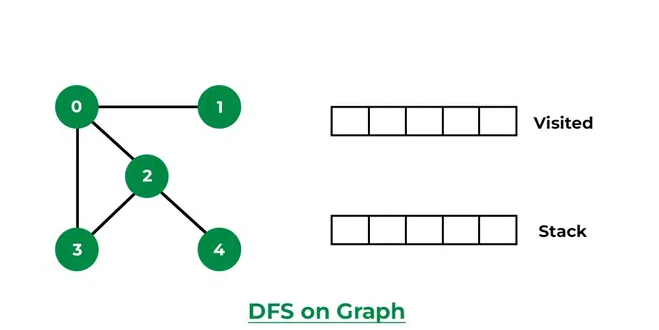
\includegraphics[width=0.75\textwidth]{images/dfs-1.png} 
    \caption{Initial condition} 
    \label{fig7:a} 
    \vspace{4ex}
  \end{subfigure}%% 
  \begin{subfigure}[b]{0.5\textwidth}
    \centering
    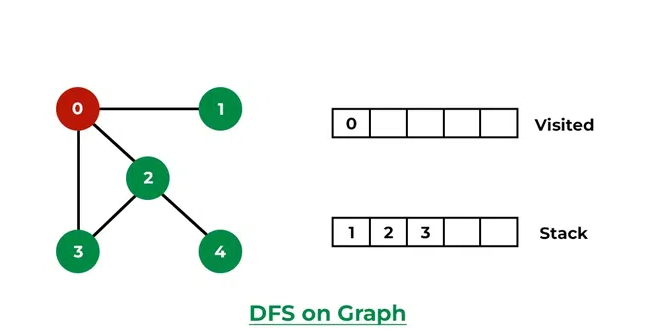
\includegraphics[width=0.75\textwidth]{images/dfs-2.png} 
    \caption{Visit the 0 vertex}  
    \label{fig7:b} 
    \vspace{4ex}
  \end{subfigure} 
  \begin{subfigure}[b]{0.5\textwidth}
    \centering
    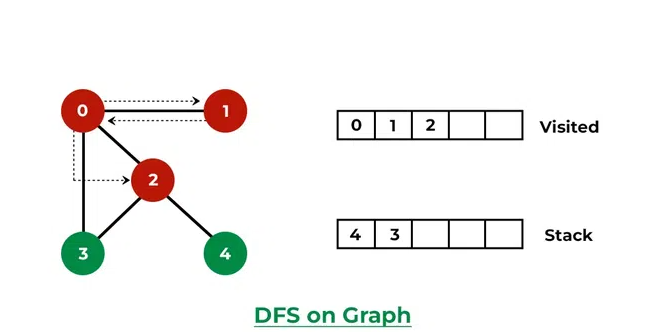
\includegraphics[width=0.75\textwidth]{images/dfs-3.png} 
    \caption{Visit 1 and 2 vertices} 
    \label{fig7:c} 
  \end{subfigure}%%
  \begin{subfigure}[b]{0.5\textwidth}
    \centering
    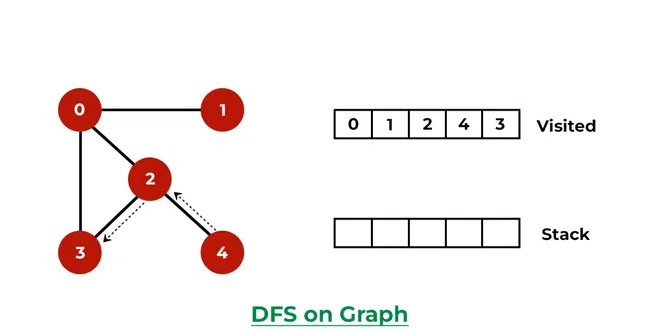
\includegraphics[width=0.75\textwidth]{images/dfs-4.png} 
    \caption{Completed condition} 
    \label{fig7:d} 
  \end{subfigure} 
  \caption{Illustration of various images}
  \label{fig:dfs} 
\end{figure}

\textbf{Depth First Search (DFS):} It operates similarly to Breadth First Search (BFS). However, instead of visiting the nodes (or links) discovered first, it explores the most recently discovered nodes. Unlike BFS, DFS can be implemented using a stack. In Figure \ref{fig:dfs}, there is a visual representation of how DFS operates while crawling a website.

The crawler begins with the root node, labeled 0, where the crawler first explores the seed URL node (0) and identifies the links within it (1, 2, and 3). Each of these links is added to the stack. The next node to be visited is node 1. Since it does not lead to any further linked nodes, the crawler proceeds to the next node in the stack, node 2. Upon visiting node 2, it becomes noticeable that it contains an additional link, denoted as 4. In contrast to BFS, which would visit node 3 in this scenario, DFS prioritizes node 4 before 3 due to its use of a stack rather than a queue. Similar to the BFS example, we use a hashmap to keep tracking the visited links to avoid loops. Like BFS, DFS has a time complexity of $O(|V|)$.

\section{Indexing}
\label{sec:indexing}
Within a search engine system, the indexer plays a crucial role in examining and structuring the content found in web pages or documents. Its primary function is to generate an index, an organized data structure that facilitates rapid and effective retrieval of pertinent information when users initiate search queries.

Inderxer breaks the content into smaller components, words, and phrases, known as tokens. Afterward, it links these tokens to the respective URLs or documents from which they were created. This structured data is then stored within the index, serving as a vital reference for the search engine. It allows the search engine to swiftly locate and present relevant search results, delivering a seamless and efficient user experience.

\subsection*{Tokenization}
Tokenization, within the context of indexing, entails fragmenting a textual document or a text string into smaller components known as tokens. These tokens are typically composed of words or subwords and are the fundamental building blocks for indexing and searching within a text. Tokenization represents a foundational and essential stage in natural language processing. A straightforward approach to tokenization involves dividing the text content based on spaces. For instance, the sentence "university of freiburg" would yield these tokens: "university", "of" and "freiburg".
While dividing text by spaces is a straightforward and convenient solution, tokenization is a more convoluted task than it initially seems. For instance, words like "Freiburg.", "Freiburg!", and "Freiburg" should be treated as a single word, "Freiburg." Additionally, words such as "write," "writes," and "writing" essentially convey the same meaning and should not be distinguished from one another. Lastly, in cases where phrases like "Freiburg-University" are connected by a hyphen, splitting solely by spaces would treat it as a single word, even though it comprises two distinct words.

Various approaches to tokenization exist, and in this thesis, each document undergoes a series of steps:

\begin{itemize}
	\item Initial text segmentation by spaces.
	\item Conversion of all words to lowercase.
	\item Removal of all special characters using regular expressions.
\end{itemize}


For example, the sentence "What! Is this the 'University of Freiburg '!" will be transformed after undergoing these processes to "what", "is", "this", "the", "of" and "freiburg". 

The regular expression used in Python is \verb|[^\w\s]+|. The regular expression \verb|[^\w\s]+| matches one or more characters that are neither word characters (letters, digits, or underscores) nor whitespace characters (spaces, tabs, line breaks). In other words, it matches any sequence of characters that contains characters other than letters, digits, underscores, spaces, tabs, or line breaks.

\subsection*{Stop Words}
Tokens such as 'the' and 'of' contribute no importance to the overall outcome of the query. Eliminating these terms via stop words can lead to excluding certain frequently used words from the indexing process. A stop words list is a list that holds words that can be excluded from the indexing process. Selecting appropriate stop words can enhance search retrieval by using a more compact indexer while also allowing user queries to bypass terms contained in the stop words list. The exclusion of stop words from the indexer can result in more relevant search results, as the search engine can direct its attention to the informative words within the documents.
\subsection*{Document Unit}
The term "document" frequently mentions the specific information intended for retrieval from a webpage. While, in some instances, this term encompasses the entirety of a page's content, this holds primarily for Universal crawlers like Google. However, in the case of the Preferential crawler employed in this thesis, the definition of a document unit is adjustable, depending on the nature of the website and the specific data the user aims to collect. For instance, the document unit may be viewed as a single product listing on an E-commerce website featuring product titles, prices, and descriptions. Contrarily, a news website might treat each article as an individual document. The chapter \ref{chap:approach} will provide more comprehensive guidance on creating a template corresponding to a document.

\subsection*{Inverted index}
As we discussed, crawlers are responsible for collecting data from the web and preparing it for users to search. Let us define "q" as the query string provided by the user and "D" as the number of documents the user attempts to search for that query. If we were to implement a simple solution, we would need to iterate over each term in "q" and then search each term against every document, each of which contains |D| terms. This approach results in a cubic complexity of O(|q| * D * |D|), which is inefficient. Implementing an inverted index is a more efficient solution to address this issue. An inverted index or inverted file is a data structure used in information retrieval systems, particularly in search engines, to store and efficiently retrieve information about the occurrences of terms (words or phrases) within a collection of documents. It is called "inverted" because it inverts the relationship between terms and documents.
In an inverted index, each unique token in the collection of documents is treated as a key, and the value associated with each token is a list of references to the documents where that token appears. This list of references allows for rapid access to all the documents containing a specific token. Some inverted indexes also include the position of the token in the document. 

Creating an Inverted index requires the next steps. The first step is to collect the documents to be indexed. In the context of this thesis, the documents referred to the content inside the crawled pages. The second step is to tokenize the text, turning each document into a list of words known as tokens. The last step is to create a dictionary that maps each term with a list of the ids of the documents that occurred. The tokenized terms are called dictionaries, and the list of ids is called postings. 

\begin{figure}[h]	
     \centering
     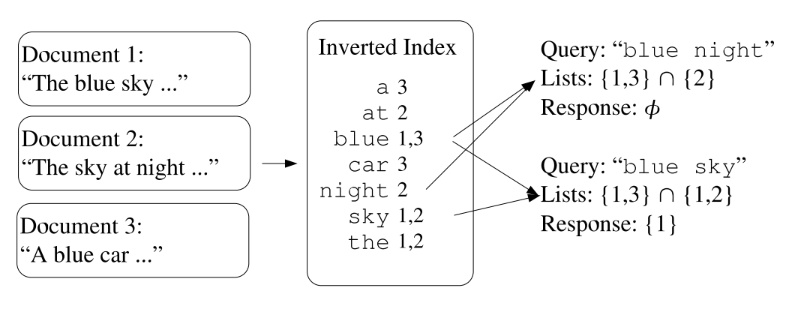
\includegraphics[width=10cm]{images/inverted_index.png}
     \caption{
An illustration of an inverted index featuring three documents. All tokens are included in this example, and the sole text normalization applied is converting all tokens to lowercase. Queries that involve multiple keywords are resolved using set operations. [3]}
     \label{fig:google-arch}
\end{figure}

Given that the inverted list can be implemented as a hashmap or dictionary in Python, where the average time complexity of a hashmap operation is O(1), the process of finding all the documents containing the query |q| has an overall time complexity of O(|q| * 1), which simplifies to O(|q|). The next step involves merging the resulting documents for each term in the query q. The time complexity of merging two sorted lists is O(n + m), where "n" is the length of the first list, and "m" is the length of the second list. Since there will be a resulting list for each term in the query q, the number of lists to merge is |q|. Consequently, the time complexity of the inverted list becomes 𝑂( |𝑞| ∗ |𝐿|), where |𝐿| represents the average length of the posting list.

It is worth noting that both |q| and |L| are typically small. The essential advantage of using the inverted list is that it makes indexing independent of the document length |D|, significantly improving performance.

\section{Ranking}
\label{sec:ranking}
As discussed, the indexing process prepares a hashmap that can be looked up to find relevant terms that match the search query; however, one needs to rank the returned result based on relevance. For example, a user searching for "what is Freiburg?" will be expecting a result about Freiburg and not to return all documents that contain tokens like "what" and "is", which are less important than the most informative term in the sentence which is "Freiburg". There are many algorithms for document ranking. However, in this thesis, BM25 will be adopted. 

\begin{equation}
BM25\_score = tf^*.\log_2(\frac{N}{df})
\label{eq:depth}
\end{equation}
\begin{equation}
tf^* = \frac{tf.(k+1)}{k.\alpha+tf}
\label{eq:depth}
\end{equation}
\begin{equation}
\alpha = \frac{1-b+b.DL}{AVDL}
\label{eq:depth}
\end{equation}

\textit{N} = Total number of docuemnts, \textit{tf} = term frequency, the number of times a word occurs in a document, \textit{df} = docuemnt frequency, The number of documents containing a particular word, \textit{DL} = document length, \textit{AVDL} =
average document length (measured in number of words).

Parameter b prevents the impact of document length normalization. It is a numeric value within the range of 0 to 1. When "b" is set to 0, there is no normalization, implying that longer documents do not face any penalties. In contrast, a value of 1 indicates complete normalization, where longer documents are penalized in proportion to their length. The default value will be set in the implementation is 0.75.

The parameter "k" governs the impact of term frequency saturation in scoring. It is a positive parameter that dictates the speed at which the term frequency component of the score achieves its peak value. When "k1" is set to 0, there is no consideration of term frequency, implying that the score remains unaffected by the number of times query terms appear in the document. On the other hand, when "k" is set to a significant value, more weight is given to term frequency, and the score escalates linearly with term frequency. The default value will be set in the implementation is 1.75.

The following example dives into the details of the BM25 equation and how it impacts ranking. Table \ref{table:bm25-documents} shows a list of documents as an example of an input to be indexed and ranked against different search queries. We start by calculating the variables needed to find the BM25 scores for each term in a document.    

Given that we have three documents, we set the variable "N" to 3. In the next step, we calculate each document's length (DF), resulting in {1: 26, 2: 21, 3: 49}. The average document length (AVDL) is determined to be 32. Substituting these values into the equation, we obtain the inverted list shown in Table \ref{table:bm25-result}.

\begin{table}[ht] 
{\footnotesize
\begin{tabular}{ P{2.5cm} ||P{11.1cm}  }      % centered columns (3 columns) 
 \hline \hline
Document ID & Document content\T\B 
\\ 
\hline
1 & The University of Freiburg, officially the Albert Ludwig University of Freiburg, is a public research university located in Freiburg im Breisgau, Baden-Württemberg, Germany.\T\B 
\\ 
\hline
2 & Freiburg im Breisgau, usually called simply Freiburg, is an independent city in the state of Baden-Württemberg in Germany.\T\B 
\\ 
\hline
3 & A university from Latin universitas 'a whole' is an institution of higher (or tertiary) education and research which awards academic degrees in several academic disciplines. Universities typically offer both undergraduate and postgraduate programs. In the United States, the designation is reserved for colleges that have a graduate school.\T\B 
\\ 
\hline \hline
    \end{tabular}
}
  \captionsetup{justification=centering,margin=2cm}
  \caption{Documents content used as an example of MB25 ranking.}
  \label{table:bm25-documents}
\end{table}

When we analyze the data in Table \ref{table:bm25-result}, it becomes evident that tokens shared by all three documents, such as 'the,' 'of,' and 'is,' have corresponding scores of 0. When dealing with common search terms, assigning lower importance or weight to the search query is advisable. For instance, users frequently search for queries like 'What is ...,' 'who is ...,' and 'Where is ...,' which include common but less informative words like 'What,' 'Who,' 'Where,' and 'is.' In such cases, the terms following these common words should be given greater value and weight.

On the other hand, unique words like 'albert' and 'ludwig' receive high scores since they are exclusive to a single document. Words such as 'freiburg' and 'university' have varying scores for each document, depending on their relative occurrences in relation to the document's length.

\begin{table}[ht] 
{\footnotesize
\begin{tabular}{ P{2.5cm} ||P{11.1cm}  }      % centered columns (3 columns) 
 \hline \hline
\textbf{Token} & \textbf{(Doc. ID, BM25 Score)}\T\B 
\\ 
\hline
the & (1, 0.0), (2, 0.0), (3, 0.0) \T\B 
\\ 
\hline
university &  (1, 1.071), (3, 0.466) \T\B 
\\ 
\hline
of  &  (1, 0.0), (2, 0.0), (3, 0.0) \T\B 
\\
\hline
freiburg  &  (1, 1.071), (2, 0.975) \T\B 
\\ 
\hline
officially  &  (1, 1.740) \T\B 
\\ 
\hline
albert  & (1, 1.740)\T\B 
\\ 
\hline
ludwig  &  (1, 1.740) \T\B 
\\ 
\hline
is  & (1, 0.0), (2, 0.0), (3, 0.0) \T\B 
\\ 
\hline
a  & (1, 0.642), (3, 0.885) \T\B 
\\ 
\hline
public  &  (1, 1.740) \T\B 
\\ 
\hline \hline
    \end{tabular}
}
  \captionsetup{justification=centering,margin=2cm}
  \caption{The first ten tokens from the resulting inverted index and the corresponding document scores. }
  \label{table:bm25-result}
\end{table}

A user's query for 'university of Freiburg' will yield the following results: (1, 2.142), (2, 0.975), (3, 0.466). The initial document with ID 1 receives the highest score since it encompasses both of the query terms. This outcome aligns with expectations, given that the first document is indeed about the University of Freiburg.

However, the concern regarding relevancy lies in the two primary keywords, "university" and "Freiburg," mentioned in documents 2 and 3. The question then becomes, which one should be prioritized in this scenario? This distinction can be influenced by adjusting the values of the "b" and "k" parameters. In this case, document 2 takes importance over document 3 because the term "Freiburg" is repeated twice, and the document itself is shorter than document 3.

The subsequent section will delve into how one can further refine the document ranking process.


\subsection{Fuzzy search}
As previously explained, the generated inverted index will contain a list of the tokens found on each document, and to find the most relevant document to the user query would be simply to split the query into tokens and search for each token and find its exact matching in the inverted index, then rank the results based on the BM25 scores. Assuming that users will not make any misspelling errors is a hard assumption, especially for some English words; there are differences between British and American spelling, for example, 'color' and 'colour'. Both have the exact same meaning with a different spelling. It would be bad not to return any result if the user chose one word over the other. Other scenarios can also be that the user is not sure about the spelling. For example, 'Freiburg' can be written as 'Frieburg'.  

Fuzzy search is a technique used in natural language processing (NLP) and information retrieval to find approximate matches for a given query or search term, even when the exact spelling or wording might not be present in the target text. This is particularly useful when dealing with typos, misspellings, variations in phrasing, or other types of small deviations from the original text.

Fuzzy search algorithms typically involve techniques like Levenshtein distance (edit distance), which calculates the minimum number of single-character edits (insertions, deletions, substitutions) required to change one string into another. Other techniques include using phonetic algorithms to find similar-sounding words, or tokenization and comparison of word n-grams to identify overlapping substrings.

Considering two character strings, s1 and s2, the edit distance that separates them represents the minimal count of edit operations needed to transform s1 into s2. The typical edit operations permitted for this purpose encompass: (i) the insertion of a character into a string, (ii) the deletion of a character from a string, and (iii) the replacement of a character within a string by another character. In the context of these operations, the term "Levenshtein distance" is sometimes used interchangeably with edit distance. To illustrate, the edit distance between "cat" and "dog" is 3. It's worth noting that the concept of edit distance can be extended to encompass varying weights assigned to different types of edit operations. For instance, assigning a greater weight to the replacement of the character "s" with "p" compared to its replacement with "a" (with the latter being physically closer on the keyboard) can be explored. This weight assignment strategy, dependent on the probability of letter substitutions, proves highly effective in practical scenarios. Nonetheless, the subsequent discussion primarily concentrates on scenarios where all edit operations bear identical weights [5].

Fuzzy search can be used with q-gram to find how similar words are.  For a string x, and an integer q ∈ N, the multiset of q-grams, denoted by Q q(x), , consists of all substrings of length q 3("freiburg") = { "fre", "rei", "eib", "ibu", "bur", "urg" }
We define it as a multiset because the same q-gram may occur multiple times and we want to know when it does 

Q 3("ababa") = { "aba", "bab", "aba" }

The number of q-grams of a string x is:

|Q q(x)| = |x| - q + 1

Similar words have many q-grams in common, that's why it can be used to find similar words. 
Lemma: for strings x and y: |Q q(x) \ Q q(y)| ≤ q ∙ ED(x, y)
Understand: A \ B denotes the set difference, that is, the elements of A without the elements from B If B is very similar to A, then A \ B is small [13]
Example:
x = freiburgerin, y = breifurgerin, ED(x, y) = Q 2(x) = { fr, re, ei, ib, bu, ur, rg, ge, er, ri, in } Q 2(y) = { br, re, ei, if, fu, ur, rg, ge, er, ri, in } 
Q 2(x) \ Q 2(y) = {fr, ib, bu}
|Q 2(x) \ Q 2(y)| = 3

To implement fuzzy search with q-gram, one can use Q-gram index. For each q-gram of a string from D, store an inverted list of all strings from D containing it, sorted lexicographically

\$fr : frankfurt, freiburg, freetown, fresno, …

More information about the implementation will be discussed in the approach section.

    \chapter{Approach}
\label{chap:approach}
This chapter introduces the distinctive concept of a configurable search engine and outlines the comprehensive software architecture. It thoroughly explores and showcases all the required components for constructing the search engine, along with discussing implementation specifics. This encompasses the pivotal models and classes employed for the components and algorithms.
Furthermore, the chapter delves into the user interface, clarifying how it enhances user experience and facilitates configuring the search engine.

\section{Software Architecture}

Figure 4 provides an overview of the software architecture employed by the search engine. Microservices architecture was used to make scalability easier and also to split the responsibilities of each component. Docker is used to enforce this architectural pattern where the Ubuntu:18.04 image is used for each component. Below is a compilation of the utilized technology stack:

\begin{figure}[h]	
     \centering
     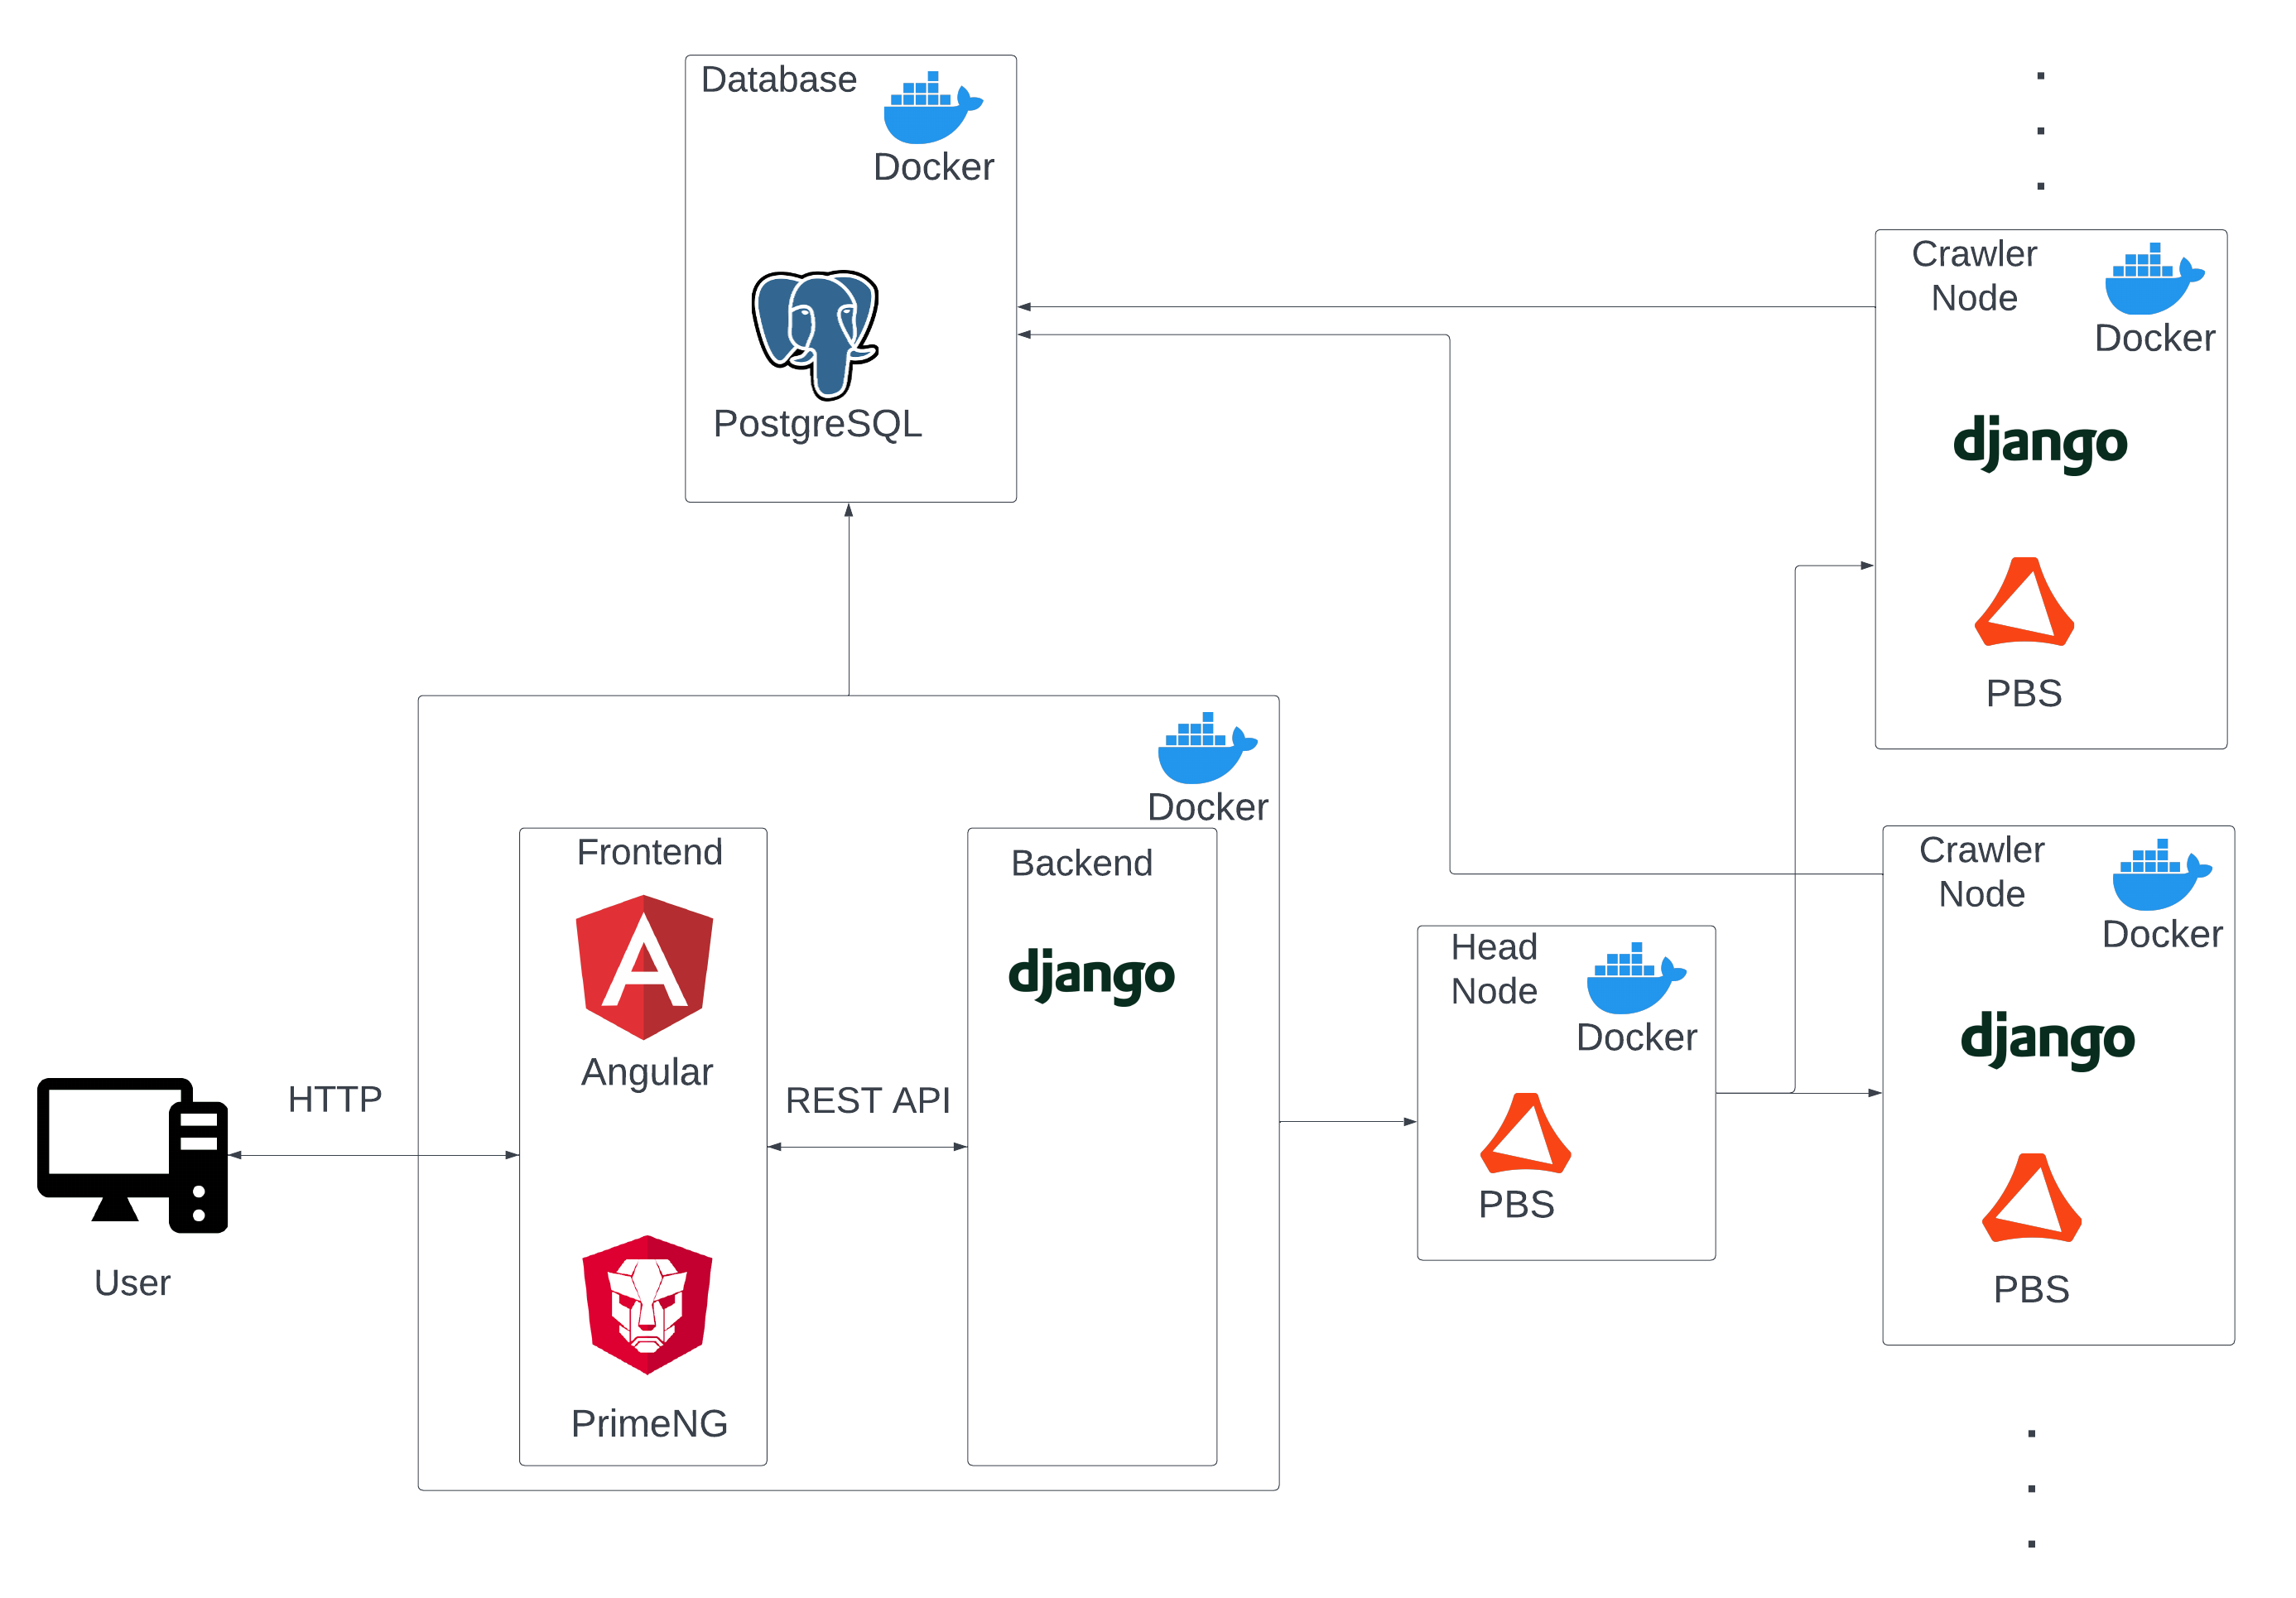
\includegraphics[width=10cm]{images/software_arch.png}
     \caption{High-level view of the software archtiticture.}
     \label{fig:software-arch}
\end{figure}

\begin{itemize}
  \item \textbf{Frontend (Angular \& PrimeNG)}: Positioned closest to the user, this component encompasses all pages and views. Angular is leveraged in conjunction with the contemporary CSS library, PrimeNG. To communicate with the backend, it employs the REST API.
  \item \textbf{Backend (Django)}: Serving as the core intelligence of the search engine, the backend houses both the crawler and indexer modules. It facilitates interaction with the Head node to initiate crawling based on user-defined configurations. Moreover, it establishes a connection with PostgreSQL for the storage of crawler and indexer configurations, along with job-related information.
  \item \textbf{Head Node (PBS)}: Operating as the central hub, this node orchestrates job management and determines the allocation of tasks to Crawler nodes, which are responsible for traversing the specified websites.
  \item \textbf{Crawler Node (PBS)}: These instances are designated to execute the crawling process and store the resulting data in the PostgreSQL database.
\end{itemize}

The application setup initiates with a minimal requirement of four microservices to operate the entire search engine. One Docker container containing both Angular and Backend logic must establish connections with two other containers: the Database and PBS Head Node. The PBS Head Node, in turn, should connect to one or more Crawler Node containers responsible for executing the crawling task. The Crawler Node will perform the crawling job and save the results to the shared Database.

The workflow begins with a user-friendly interface presented by Angular and PrimeNG, encompassing all the configurations and tools enabling users to crawl quickly and index various websites. Users can modify configurations and submit a crawling job to the Head Node. The Head Node, in response, identifies an available Crawler Node to execute the task. It's worth noting that the PBS cluster can be bypassed, and the crawling process can be run locally on a localhost server. Users can monitor the progress of the running job from the browser. Once crawling is completed and the user is happy with the result, the user can start indexing. The indexing job also does not support a distributed architecture and will be executed locally and not on the PBS cluster.


\section{Crawler Implmentation}

PBS Crawler Node runs the crawling job or can also run locally. The job supports multithreading. As illustrated by the pseudo-code shown in Algorithm [1], the crawler starts by loading the configuration submitted by the user from the Database. More details about the configuration are in the user interface section. Based on the configuration of a thread pool, the number of threads is read by the configuration. The thread pool contains all the threads crawling the site, where each thread contains a queue of URLs that it crawls from. The thread pool makes sure that if one thread has no URLs anymore, it can ask other threads to help. Algorithm [2] explains how this sharing URLs mechanism works. 


\begin{algorithm}[H]
	\caption{Start Crawling}\label{alg:alg1}
	\begin{algorithmic}[1]
		\State load\_crawler\_configurations()
		\State $thread$ $\gets$ create\_threads\_pool()
	    \State $urls\_queue$ $\gets$ get\_thread\_urls\_queue($thread)$)
	    \State $seed\_url$ $\gets$ get\_seed\_url()
	    \State add\_url\_to\_queue($urls\_queue$, $seed\_url$)
	    \State $robot\_file$ $\gets$ get\_robot\_file\_content()
	    \While {$urls\_queue$ not empty or all threads not done}
		\If{$urls\_queue$ is empty}
		    \State $urls\_queue$ $\gets$ get\_thread\_urls\_queue($thread$)
		\Else
			\State $current\_url$ $\gets$ urls\_queue\_next\_url()
			\State filter\_unwanted\_urls($current\_url$)
			\State request\_page($current\_url$)
            \State execute\_automated\_actions()
			\State find\_next\_urls\_and\_add\_them\_to\_urls\_queue()
			\State $docs$ $\gets$ find\_and\_download\_targeted\_documents()
			\State filter\_unwanted\_documents($docs$)
		\EndIf
		\EndWhile

	\end{algorithmic}
\end{algorithm}


A seed URL is added to the current thread queue. The seed URL represents the starting point for the crawling, and the user configuration defines it. Using the sead url, the robots.txt content is downloaded once and can be reused for the rest of the crawling process.    

Each thread goes into an infinite loop that will continue to run either if the URLs queue still contains URLs to be fetched or at least one thread is still running. This guarantees that although one thread is running, it can be that that thread contains a lot of URLs that need help with crawling, and the free threads can share the load with it. If the thread queue is empty, it will ask the pool to find the next URLs to fetch. Otherwise, the first URL in the queue will be fetched, and a request using Selenium will be made. Afterwards, automated actions such as scrolling down, waiting and clicking defined by the user are executed. Those actions give the power to control the browser by the user to mimic real agent behaviour. The action chain will be discussed more in the User Interface section.  

After the page is rendered and the automated actions are executed, the next step is to collect the next URLs and add them to the URLs queue. The last step is to parse the documents needed from the page and filter the duplicated documents. 


\subsection{Links Data Structure}
The website's page navigation algorithm can be likened to a Level Order Traversal. The tree structure is established in the following manner: the seed URL acts as the tree's root node, representing level 0. After you explore the root page's content and gather its URLs, these URLs are assigned to the next level, level 1. Each page within level 1 is then visited, its contained URLs are collected, and these newly collected URLs are assigned to level 2. This process continues as you move deeper into the website until a maximum depth is reached, which is pre-defined by the user.
This algorithm offers an advantage in that it makes it straightforward to prioritize pages based on their respective levels. For instance, in some scenarios, pages closer to the initial seed URL may receive higher priority, potentially yielding better outcomes. In other cases, deeper pages within the structure may hold more significance than those closer to the seed URL. Choosing the proper algorithm is possible in the UI.

\subsection{Practical Challenges}
\begin{itemize}
  \item \textbf{Avoiding Loops}: Looping is when a web crawler repeatedly visits and requests the same web pages or URLs in a never-ending cycle, often resulting in excessive traffic to the same content. This is problematic as it wastes resources can also be inefficient, and can prevent the crawler from continuing. The first method to prevent looping is to record all the URLs visited and crawled. Before making a new request, we check if the URL is in this list. If it is, skip crawling it again to prevent loops. The second method is to use URL normalization. Normalize URLs by removing unnecessary components such as query parameters, fragments, or trailing slashes. This helps ensure that URLs with different representations (e.g., with and without a trailing slash) are treated as the same URL.


\item  \textbf{Duplicated Content}: While the same web crawler avoids revisiting identical URLs to prevent content duplication, it's important to note that identical content may exist in different URLs paths within the same website. For instance, a men's shoe might be accessible via various links like "/winter/shoes/", "/men/shoes/", or "/sales/shoes/". Relying solely on the URL as a unique identifier to prevent content duplication is not foolproof.
A more effective approach involves comparing the content itself with the database after parsing. Instead of a straightforward content check against the database, which can pose performance challenges, we employ a more efficient method. We generate a unique hash code using the SHA-1 hashing algorithm based on the content string intended for storage. This hash code is then stored in the database.
Before saving any new content, we can verify if the hash code already exists in the database. This method ensures content uniqueness, even when it appears under different URLs on the same site, without the computational overhead of directly comparing lengthy content strings in the database.

\item  \textbf{Dynamic Content}:Crawling dynamic websites presents a distinct set of challenges compared to static websites. Dynamic sites generate content on the client side through technologies like JavaScript, adding complexity to the task of accessing and extracting data. A primary concern lies in uncovering concealed content that necessitates user interaction. For instance, certain websites hide lengthy content portions, revealing them only upon clicking a "read more" button. Additionally, most websites implement lazy loading, fetching content on-demand via AJAX requests.
To address these challenges, Selenium establishes a genuine session and fully renders the webpage. This approach allows for emulating user interactions using action chains, which simulate actions such as waiting, scrolling, and clicking. More details regarding this can be found in the User Interface section.

\item  \textbf{Termination Conditions}: Crawlers can be brought to a halt by establishing specific criteria to ensure termination. The initial criterion involves defining a maximum depth, which restricts the number of page transitions to a single level. Additionally, monitoring and restricting the total count of visited pages and collected documents is possible. Another method is to employ a wall time measurement to monitor the crawler's runtime duration and trigger an abort if the crawler exceeds the expected time frame.

\item  \textbf{Avoiding DOS}: Increasing the number of requests and expanding the crawler's capacity by adding more threads or nodes may seem enticing to boost performance. However, this approach carries a significant risk of overwhelming the targeted servers, potentially resulting in Distributed Denial of Service (DDoS) or Denial of Service (DoS) attacks. Servers can perceive this surge in requests as an attack, which could lead to the crawler being blacklisted and subsequently banned.
To mitigate this risk, it's crucial to introduce a waiting period between each request made by the same crawler. Additionally, when using Selenium, a deliberate delay of at least one second or more is already integrated to allow for the complete rendering of web pages. Nevertheless, these precautions alone may not prevent users from adding more nodes and executing DDoS attacks. Consequently, it is strongly advisable to exercise cautious management by monitoring and regulating the number of threads and nodes. This approach demonstrates respect for the targeted servers and helps prevent overloading them.
\end{itemize}

\\

\section{Indexer Implmentation}

The indexing phase follows the crawling step, as it necessitates the downloading of documents. Unlike crawling, which can be computationally intensive, indexing is relatively lightweight. Hence, it is carried out on the localhost with multithreading support.
Algorithm [2] clarifies the indexing process. Firstly, the algorithm loads the user-defined indexing configurations. You can find more details about these configurations in the User Interface Design section. Subsequently, an empty inverted list is initialized. An inverted list is a data structure used to associate words or terms with the documents in which they appear. In Python, it can be implemented as a dictionary (Dict[str, list[int]]), where each word serves as a key, and the corresponding value is a list of document IDs containing that word.


\begin{algorithm}[H]
	\caption{Create Inverted List}\label{alg:alg1}
	\begin{algorithmic}[1]
	    \Require $documents$ not empty
		\State $config$ $\gets$ load\_indexer\_configurations()
		\State $inverted\_list$ $\gets$ init\_inverted\_list()
		\State $threshold$ $\gets$ get\_small\_words\_threshold($config$)
	    \State $stop\_list$ $\gets$ stop\_words\_list($config$)
        \For{$doc$ in $documents$}
          \State $doc\_length$ $\gets$ 0}
          \State $words$ $\gets$ tokenize($doc$)}
          \For{$word$ in $words$}
          	\State $doc\_length$ $\gets$ 0}
          	\If{$word$ > threshold and $word$ not in $stop\_list$}
		    	\State add\_word\_and\_doc\_id\_to\_inverted\_list($word$, $doc.id$)
		    	\State $doc\_length$ $\mathrel{+}=$ 1}
			\EndIf
          \EndFor
          \State add\_to\_doc\_lengths\_list($doc\_length$)
        \EndFor
        \State calculate\_bm25\_score($inverted\_list$)
        \State cache($inverted\_list$)

	\end{algorithmic}
\end{algorithm}

The user specifies three variables: "threshold" and "stop\_list," which are retrieved from the database. The "threshold" represents the minimum word length required for tokenization from a document. The "stop\_list" is a predefined list of terms that should be omitted from the indexing process.
The algorithm then iterates through all the documents, performing the following steps for each one:
Initializes the document length as a counter, initially set to zero.
Tokenizes the document to obtain a list of words.
Iterates through the word list, checking each word's length against the threshold and verifying if it is not in the stop\_list. If these conditions are met, the word is added to the inverted list, and the document length counter is incremented by one.


Once the inverted list is constructed, we calculate the MB25 score based on equation 3.4. Afterwards, it is saved into a cache for future retrieval and use.

\section{User Interface Design}
The core focus of this thesis extends beyond merely building and designing a search engine. It also encompasses the vital objective of enabling users to effortlessly configure and utilize it. In the forthcoming section, we will delve into the User Interface design, workflow, and the user-facing configurations.

The user begins their journey on the homepage, where they can access documentation explaining how to utilize the application. The application's workflow commences with the creation of templates, which serve as blueprints for specifying the document fields to be extracted from web pages. It is a prerequisite to establish a unique template for each page, although the same template can also be applied across different websites. These templates consist of components referred to as "inspectors," each comprising the following attributes:

\begin{itemize}
  \item \textbf{Name}: This denotes the inspector's identifier, such as "Price" or "Title."

\item \textbf{Selector}: It encompasses the XPath expression pinpointing the chosen element, for instance, //*[contains(@class, 'product-title')].

\item \textbf{Type}: This can assume values like "Text," "Link," or "Image," signifying the nature of the content to be extracted.

\item \textbf{Variable Name (\textit{Optional})}: This is an optional shorthand representation of the selector, facilitating its use during the indexing process to enhance search results (Ranking).

\item \textbf{Clean-up Expression List (\textit{Optional})}: Here, you can specify a regular expression utilized to refine the extracted value from the inspector. This proves beneficial in eliminating unwanted noise. A use case for this can be to remove the currency when extracting a price.

\item \textbf{Attribute (\textit{Optional})}: This field allows you to specify an HTML element attribute, such as "src," "name," or "href," as an optional parameter.
\end{itemize}


The following phase is contingent upon the specific characteristics of the website being targeted, referred to as the "Actions Chain" tab. An "Actions Chain" constitutes an array of sequenced actions that replicate user interactions. This functionality proves valuable for tasks such as acknowledging cookies, scrolling to load additional content, or patiently waiting for the website to finish rendering in cases where the process may exceed the expected duration.

\begin{figure}[h]	
     \centering
     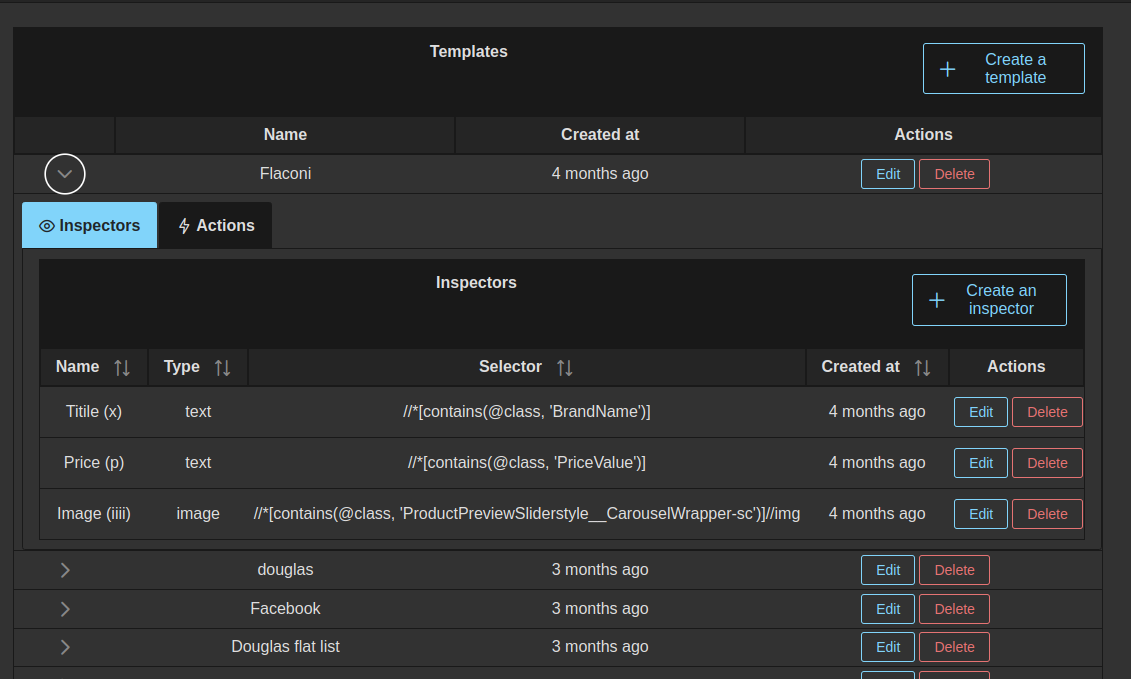
\includegraphics[width=13cm]{images/demo-3.png}
     \caption{An overview of the Templates table containing inspectors list projecting the targeted feilds in a document}
     \label{fig:software-arch}
\end{figure}

Once the Template is created, the subsequent step is to access the Crawlers page and initiate the creation of a new Crawler. A Crawler comprises various essential configurations, including:

\begin{table}[ht] 
{\footnotesize
\begin{tabular}{ P{2.5cm} ||P{11.1cm}  }      % centered columns (3 columns) 
 \hline \hline
\textbf{Attribute} & \textbf{Description}\T\B 
\\ 
\hline
\textbf{Name} & A user-defined identifier for the crawler \T\B 
\\ 
\hline
\textbf{Template} & The template utilized by the crawler to recognize HTML elements for crawling and storage \T\B 
\\ 
\hline
\textbf{Max pages} & The upper limit for the number of pages to be visited during the crawling process \T\B 
\\ 
\hline
\textbf{Max collected docs} & The maximum number of documents to be collected \T\B 
\\ 
\hline
\textbf{Max pages} & The upper limit for the number of pages to be visited during the crawling process \T\B 
\\ 
\hline
\textbf{Seed URL} & The initial URL from which the crawler will commence the crawling process. Ensure that the URL includes the protocol (e.g., https://) \T\B 
\\ 
\hline
\textbf{Robots file URL} & The URL where the robots.txt file can be located \T\B 
\\ 
\hline
\textbf{Threads} & Specifies the number of threads to be employed in the crawling process. \T\B 
\\ 
\hline
\textbf{Links Scope (Pagination)} & Defines the specific divs on which the crawler should concentrate. Typically, you'd want the crawler to avoid collecting links from areas like headers and footers. Example: //*[contains(@class, 'product-overview')] \T\B 
\\ 
\hline
\textbf{Excluded URLs} & Identifies URLs that the crawler must steer clear of and refrain from visiting. \T\B 
\\ 
\hline
\textbf{Timeout in minutes} & Sets the duration for which the crawler should continue crawling.\\ 
\hline
\textbf{Retry} & Determines how many retry attempts should be made if the crawler encounters difficulties while crawling a page. \T\B 
\\ 
\hline
\textbf{Max depth} & Establishes the depth to which the crawler should navigate through pages. \T\B 
\\ 
\hline
\textbf{Sleep} in ms & Specifies the number of milliseconds the crawler should wait before making the next request. \T\B 
\\ 
\hline
\textbf{Show browser} & This option, when enabled, displays the browser interface during crawling, which is beneficial for debugging purposes. \T\B 
\\ 
\hline \hline
    \end{tabular}
}
  \captionsetup{justification=centering,margin=2cm}
  \caption{Crawler configurations options}
\end{table}

Once you've set up the crawler with the appropriate configurations tailored to the specific website you're targeting, the next step is to create a job referred to as a "runner." Multiple runners can be associated with each crawler, allowing them to run on different days or machines. It's important to note that each runner can utilize multithreading based on the crawler's configurations and employ distinct crawler settings. This approach provides an effective means to assess the crawler's performance until the desired outcome is achieved. Every runner instance necessitates the presence of the crawler and a designated machine IP where it will execute. The chosen machine must be registered within the PBS Head Node and must be online. By default, "localhost" is set as the value, which can be employed for testing purposes and for circumventing the PBS cluster.

\begin{figure}[h]	
     \centering
     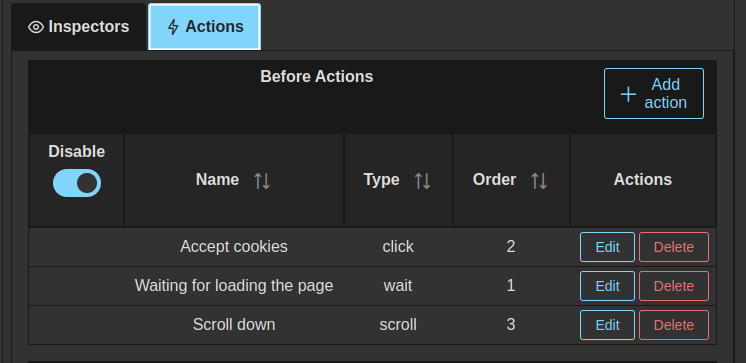
\includegraphics[width=13cm]{images/demo-5.png}
     \caption{High-level view of the software archtiticture.}
     \label{fig:software-arch}
\end{figure}


It's crucial to keep a close eye on the crawler runner to monitor its performance and configuration effectiveness before finalizing it. This proactive approach helps save time and guarantees that the crawler is collecting the accurate data. The "runners" table provides a straightforward and informative progress overview through four primary status indicators. The initial status is "New," representing the runner's initialization before the crawling process begins. "Running" signifies that the crawling process is currently underway. "Exit" indicates a status change that occurs when an error occurs, leading to the termination of the crawling process. Finally, "Completed" marks the last status, indicating that the runner has finished its task and exited. During the crawling process, various statistics about the runner are gathered, including information such as the total number of visited pages, the average number of documents discovered per page, and the various HTTP status codes encountered.


\begin{figure}[h]	
     \centering
     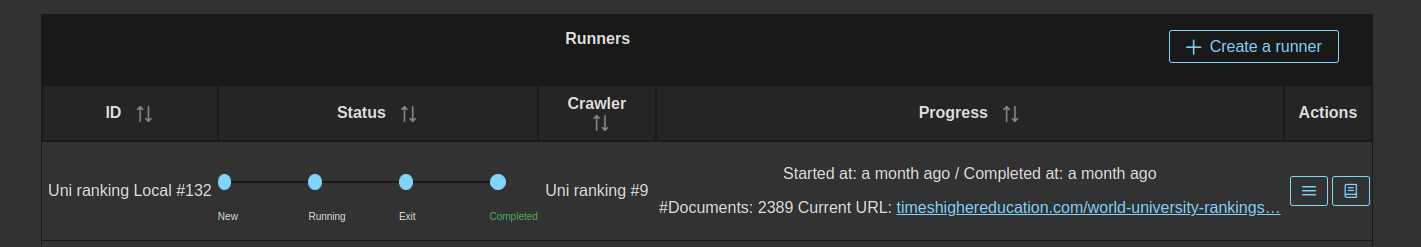
\includegraphics[width=13cm]{images/demo-8.png}
     \caption{High-level view of the software archtiticture.}
     \label{fig:software-arch}
\end{figure}


\begin{figure}[h]	
     \centering
     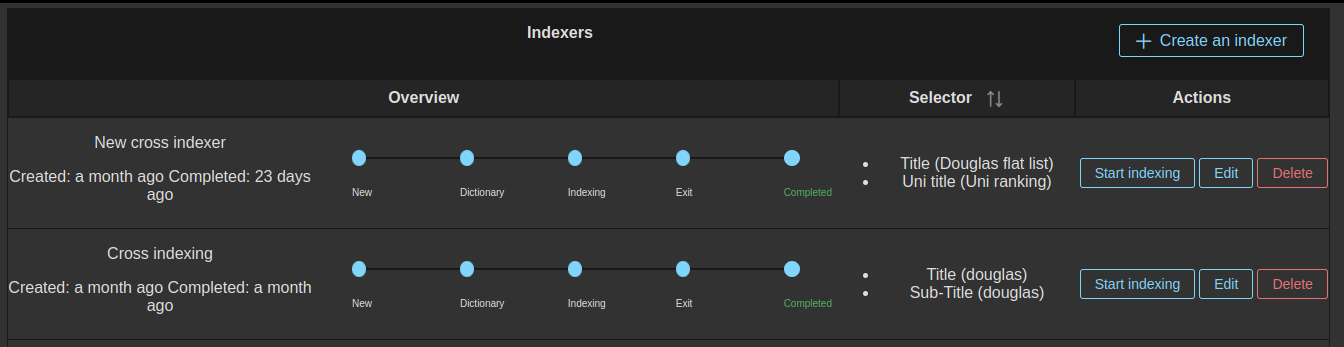
\includegraphics[width=13cm]{images/demo-10.png}
     \caption{High-level view of the software archtiticture.}
     \label{fig:software-arch}
\end{figure}


\begin{figure}[h]	
     \centering
     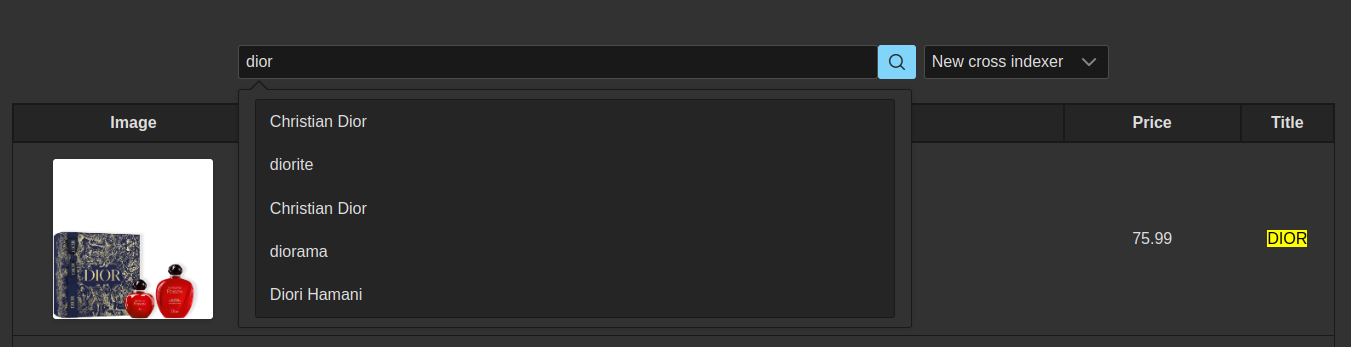
\includegraphics[width=13cm]{images/demo-12.png}
     \caption{High-level view of the software archtiticture.}
     \label{fig:software-arch}
\end{figure}
    \chapter{Evaluation}
\label{chap:evaluation}
In this chapter, our objective is to assess and examine the existing search engine implementation. The evaluation process is structured into three primary segments: Crawler, Indexer, and User Experience.

\section{Testing Environment}
The evaluation procedure is significantly influenced by the specific computing device executing the tests. Displaying information about the testing machine utilized can provide enhanced clarity and facilitate meaningful comparisons.


\begin{table}[ht] 
{\footnotesize
\begin{tabular}{ |p{2.5cm}||p{10.3cm}|  }
 \hline \hline
\textbf{Operating System} & Ubuntu 22.04.3 LTS \T\B 
\\ 
\hline
\textbf{CPU} & Intel(R) Core(TM) i7-10510U @ 1.80GHz; 4 cores; 8 threads \T\B 
\\ 
\hline
\textbf{RAM} & 32GB\T\B 
\\ 
\hline
\textbf{Machine} & Lenovo ThinkPad P15s Gen 1\T\B 
\\ 
\hline \hline
    \end{tabular}
}
  \captionsetup{justification=centering,margin=2cm}
  \caption{Local machine setup}
\end{table}

\section{Crawler}  

To evaluate the web crawler, the following criteria can be employed for measurement:


{\renewcommand\labelitemi{}
\begin{itemize}
  \item \textbf{Coverage}: This metric measures the proportion of relevant web pages that the crawler can locate and fetch from the internet.

  \item \textbf{Scalability}: It evaluates the crawler's facility for efficiently scaling up to add more computing power to crawl more content.

  \item \textbf{Versatility}: Can the crawler be applied to explore diverse types of content from various websites, encompassing text, multimedia, and links?

  \item \textbf{Robustness}: The crawler's ability to adeptly manage challenging scenarios and errors.

  \item \textbf{Politeness}:  the extent to which the crawler respects the rules and policies of the web servers and avoids overloading them with requests and forbidden links.

\end{itemize}

\subsection{Datasets} 
Evaluating a web crawler necessitates the utilization of a static website as a reliable reference point. The crawler-test\footnote{\url{https://crawler-test.com/}} website serves as an excellent choice for this purpose due to its diverse range of content and links, containing a wide range of scenarios that a crawler might encounter. This website effectively employs robots.txt to provide guidance to the crawler, allowing for an assessment of its politeness. Moreover, it includes a section containing links that yield various HTTP request status codes, such as 4xx and 5xx, which proves valuable for ensuring the crawler's robustness. Additionally, it incorporates multiple instances of page redirection, including scenarios like infinite redirection, which serves the dual purpose of evaluating the crawler's ability to avoid traps and enhancing its overall resilience.

To enhance the coverage and versatility of our crawler testing, we are considering two additional websites encompassing a broader range of use cases, ensuring that the crawler can effectively handle various HTML structures and more generic scenarios.
The first use case involves extracting product information from an E-commerce platform like Douglas\footnote{\url{https://www.douglas.de/}}. This website offers over 160,000 diverse products, making it an ideal candidate for testing different content types, including images. We will categorize our testing into three distinct datasets: small (with 100 products), medium (with 1,000 products), and large (with 10,000 products) to evaluate the crawler's performance under different data sizes thoroughly.
The second website, Times Higher Education\footnote{\url{https://www.timeshighereducation.com/world-university-rankings/2023/world-ranking}}, specializes in annually ranking universities. This unique characteristic allows us to evaluate content changes occurring on a yearly basis, setting it apart from other websites that undergo daily alterations, which can prove challenging for accurate evaluation.

\subsection{Experiments}
The crawler-test website is selected to assess and experiment with various crawler configurations. This choice is attributed to its stable, non-changing nature, which facilitates straightforward and meaningful comparisons of results across different configurations.
 
The first testing case is the coverage. It is vital to ensure the crawler can find the links inside the page, navigate to them and crawl them. 

Table \ref{table:crawler_test_config} displays the testing configurations used in the experiment. The Seed URL serves as the initial point from which the crawler begins its procedure, set to the root path of the crawler-test. The "Allow Multi Elements" checkbox is disabled (set to False) because the objective is not to gather a list of documents; each page contains a single text field. The Max Pages parameter is configured to a limit of 500, ensuring that the crawler does not exceed this number of pages. This figure can be adjusted based on the website's size to be crawled; for instance, smaller websites with around 50 pages may require a lower limit. The number of threads is set to the default value of 1.
We have set the Max Depth to 1 to enable easier coverage testing. This choice allows for easier comparison between the number of visited pages and the number of URLs discovered in the site's root path, which, upon simple page inspection, contains 415 links. Since the expected maximum number of pages is 415, the Max Docs parameter can be constrained to 500.
The inspectors are set to target the content of each page; thus, one inspector is only needed. No automated actions, such as scrolling or waiting, are necessary for this use case; therefore, they can be left. Any properties not explicitly mentioned can be left at their default settings.

\begin{table}[ht] 
{\footnotesize
\begin{tabular}{ |p{2.5cm}||p{10.3cm}|  }
 \hline \hline
\textbf{Seed URL} & \href{https://crawler-test.com/}{https://crawler-test.com/}\T\B 
\\ 
\hline
\textbf{Allow Multi Elements} & False \T\B 
\\ 
\hline
\textbf{Max Pages} & 500\T\B 
\\ 
\hline
\textbf{Threads} & 1\T\B 
\\ 
\hline
\textbf{Max Depth} & 1\T\B 
\\ 
\hline
\textbf{Pagination} & None\T\B 
\\ 
\hline
\textbf{Actions} & None\T\B 
\\ 
\hline
\textbf{Inspectors} & //*[contains(@class, 'large-12 columns')]\T\B 
\\ 
\hline
\textbf{Max Docs} & 500\T\B 
\\ 
\hline \hline
    \end{tabular}
}
  \captionsetup{justification=centering,margin=2cm}
  \caption{Crawler configuration}
  \label{table:crawler_test_config}
\end{table}

After creating a runner that runs, starts the crawling process and is completed, the result of the crawler should be similar to the one shown in Table \ref{table:crawler_test_result}. Looking at the Links row, we can note that the crawler found 406 out of the expected 415 links. This is normal as the crawler will normalize all the found links, including skipping the link fragments, duplicated links and any broken links. 402 pages out of 406 found links are crawled correctly. The other four pages are categorized as Cross Site links, meaning they do not belong to the Seed URL hostname crawler-test.com. This is important to evaluate to ensure that the crawler stays focused, does not jump to sites out of the intended scope, and does not spend valuable resources. Already Visited links is a counter that checks how many times the crawler found a link that has already been visited and skipped, in this case, 0. When no multithreading is used, and the Max Depth is only set to 1, the Already Visited is expected to be 0 because the duplicated links will be already excluded in the normalizing process before starting to crawl. 


\begin{table}[ht] 
{\footnotesize
\begin{tabular}{ |p{2.5cm}||p{10.3cm}|  }
 \hline \hline
\textbf{Links} & Collected: 406/415 . Visited Correctly: 402. Cross Site: 4 . Already Visited: 0\T\B 
\\ 
\hline
\textbf{Time} & Tot. Spent: 671.19 s. Avg. Processing: 1.68 s. Avg. Page Rendering: 0.697 s\T\B 
\\
\hline
\textbf{Status Codes} &   101: 1  102: 1  200: 321  201: 1  202: 1  203: 1  206: 3  207: 1  226: 1  300: 1  305: 2  306: 1  400: 1  401: 1  402: 1  403: 2  404: 11  405: 1  406: 1  407: 1  408: 1  409: 1  410: 1  411: 1  412: 1  413: 1  414: 1  415: 1  416: 1  417: 1  418: 1  419: 1  420: 1  421: 1  422: 1  423: 1  424: 1  426: 1  428: 1  429: 1  431: 1  440: 1  444: 1  449: 1  450: 1  451: 1  494: 1  495: 1  496: 1  497: 1  498: 1  499: 1  500: 2  501: 1  502: 1  503: 1  504: 1  505: 1  506: 1  507: 1  508: 1  509: 1  510: 1  511: 1  520: 1  598: 1  
599: 1\T\B 
\\ 
\hline
\textbf{Docs \& Content} & Tot. Docs Found: 255. Duplicated Content:24. Avg. Docs Per Page:1. Average page size: 0.000346\T\B 
\\ 
\hline
\textbf{Robots.txt Exists} & True\T\B 
\\ 
\hline
\textbf{Tot. Errors} & 6\T\B 
\\ 
\hline \hline
    \end{tabular}
}
  \captionsetup{justification=centering,margin=2cm}
  \caption{Crawler configuration}
    \label{table:crawler_test_result}
\end{table}


Evaluating the performance of a web crawler is challenging as it depends on different aspects, such as the page's size and how fast the page loads. Moreover, if the site uses pagination, this can add extra waiting time to render the rest of the content. However, some valuable matrices can be helpful to give a good insight like those shown in the Time row. The total time spent to crawl 406 pages took approximately 11 minutes. To give a better perspective, the enterprise solution Parsehub \footnote{\url{https://www.parsehub.com/pricing}} the free teer without IP Rotation, can crawl 200 pages in 40 minutes, and the Standard expensive teer with IP Rotation that costs \$189 can crawl 200 pages in 10 minutes. This means crawling the 406 pages inside the crawler-test will take 20 minutes. Comparing the crawler with the Standard tier, it is faster by 2X. Note that in this evaluation, the performance can be increased by using more threads or nodes to distribute the loads, which we will evaluate. 

While some crawlers, such as the one described in the following paper \cite{shkapenyuk2002design}, can achieve crawling rates of up to 300 pages per second, this comparison is not applicable. Crawling 300 pages from the same domain, as we are doing, is more challenging than simply crawling 300 different pages from 300 different websites. Distributing 300 HTTP requests evenly across these 300 websites is acceptable and does not result in a Denial of Service (DoS) issue because each domain receives only one request per second. However, in the context of Scribueg, users aim to target a specific set of websites, which could include just one website. If we send 300 requests to the same website, it could overload and crash the site.

\lstset{language=HTML}
\begin{lstlisting}[frame=single, caption={The dynamically-inserted-text link content before rendering},captionpos=b, label={lst:no_rendering}]
<body>
  <h1 id="h1"></h1> 
  <p id="par"></p>
  <script>
    var title = 'Some random text';
    var content = 'Some long content ...'; 
    document.getElementById("h1").innerHTML = title; 
    document.getElementById("par").innerHTML = content;
  </script>
</body>
\end{lstlisting}

Improving the average page rendering time (0.679) is achievable by avoiding using rendering engines like Selenium. Processing a simple HTTP request is often quicker than rendering the entire page. However, it's essential to note that the rendering step is crucial in handling dynamic content. For instance, consider the dynamically inserted text, indicated by the link \footnote{\url{https://crawler-test.com/javascript/dynamically-inserted-text}}. This link is a straightforward example to illustrate the significance of the rendering process for web crawlers.
Using a simple wget command in Linux, you can download the content depicted in \ref{lst:no_rendering}. This content reveals that the two HTML tags, h1 and p, lack the inner text that the crawler can collect as a document. Although there's a script tag designed to replace the innerHTML for each tag with text, without a rendering engine, the JavaScript logic remains unexecuted. Consequently, gathering the inner text of these tags becomes an impossibility. On the other hand, \ref{lst:rendered} shows the same page content after rendering where both tags are updated, and both contain the right content that the crawler can see and download.
While this is a simplified example, it's easy to visualise more complicated websites employing advanced JavaScript frameworks and libraries for client-side rendering. This complexity increases the rendering time due to the execution of all JavaScript logic and the subsequent updating of the HTML DOM. Given that the crawler's objective is to locate and collect all HTML content, striking a balance between efficiency and comprehensiveness is a challenge that must be addressed.

\lstset{language=HTML}
\begin{lstlisting}[frame=single, caption={The dynamically-inserted-text link content after rendering},captionpos=b, label={lst:rendered}]
<body>
  <h1 id="h1">
    'Some random text'
  </h1> 
  <p id="par">
    'Some long content ...'
  </p>
  <script>
    var title = 'Some random text';
    var content = 'Some long content ...'; 
    document.getElementById("h1").innerHTML = title; 
    document.getElementById("par").innerHTML = content;
  </script>
</body>
\end{lstlisting}

The Status Codes metric reveals the variety of distinct status codes encountered while crawling. Given that this website serves as a testing ground for various scenarios, it naturally exhibits a range of status codes. Evaluating the crawler's resilience across these diverse cases is vital for enhancing its stability. Notably, the crawler should remain operational even when encountering a status code other than 200.
In the specific test case, it's worth noting that the crawler confronted 66 different status codes without terminating and completed the crawling operation. This outcome encompasses status codes from the 1xx, 2xx, 3xx, 4xx, and 5xx ranges.

The "Docs \& Content" section provides information regarding the collected and downloaded content. The "Tot. Docs found" metric indicates that 255 documents have been successfully downloaded. Among these, 25 documents are duplicates. This duplication is intentional, as this testing site contains repetitive information designed to verify the functionality of this feature.
The "Avg. Docs per page" value is 1, indicating that the site typically presents one document per page. The presence of the "Robots.txt Exists" flag covers the commitment to polite crawling behaviour. The flag is set to True when this file is located and successfully downloaded. It's essential to emphasize the importance of respectful crawling and commitment to the Robots.txt file protocol.
Lastly, the "Tot. Errors" metric accounts for various Selenium exceptions\footnote{\url{https://www.selenium.dev/selenium/docs/api/py/common/selenium.common.exceptions.html}} that may arise during the crawling process. As mentioned, many errors are expected since this is a testing site with different edge cases, and not terminating under those conditions is a good sign.


Checking if changing thew depth will increase the coverage.


The next step is to evaluate if the crawler jumps between pages and can increase the coverage. We will change the Max Depth from 1 to 10 to evaluate this. This will allow the crawler to jump up to 10 levels deeper, collecting more links and documents. Table \ref{table:crawler_test_config_depth_10} shows the configurations used for this test case. 

Unfortunately, knowing exactly how many links the crawler-test site contains is challenging. However, since we have evaluated how the crawler behaves when the Max Depth is, one can give some assurance on the rest of the results. The table \ref{table:crawler_test_result_depth_10} shows 895 links has been found which was expected as the depth of the crawler has increased from 1 to 10. 


\begin{table}[ht] 
{\footnotesize
\begin{tabular}{ |p{2.5cm}||p{10.3cm}|  }
 \hline \hline
\textbf{Seed URL} & \href{https://crawler-test.com/}{https://crawler-test.com/}\T\B 
\\ 
\hline
\textbf{Allow Multi Elements} & False \T\B 
\\ 
\hline
\textbf{Max Pages} & 1000\T\B 
\\ 
\hline
\textbf{Threads} & 1\T\B 
\\ 
\hline
\textbf{Max Depth} & 10\T\B 
\\ 
\hline
\textbf{Pagination} & None\T\B 
\\ 
\hline
\textbf{Actions} & None\T\B 
\\ 
\hline
\textbf{Inspectors} & //*[contains(@class, 'large-12 columns')]\T\B 
\\ 
\hline
\textbf{Max Docs} & 1000\T\B 
\\ 
\hline \hline
    \end{tabular}
}
  \captionsetup{justification=centering,margin=2cm}
  \caption{Crawler configuration}
    \label{table:crawler_test_config_depth_10}
\end{table}

The next step is to evaluate if the crawler jumps between pages and can increase the coverage. We will change the Max Depth from 1 to 10 to evaluate this. This will allow the crawler to jump up to 10 levels deeper, collecting more links and documents. Table \ref{table:crawler_test_config_depth_10} shows the configurations used for this test case. 

Unfortunately, knowing exactly how many links the crawler-test site contains is challenging. However, since we have evaluated how the crawler behaves when the Max Depth is, one can give some assurance on the rest of the results. The table \ref{table:crawler_test_result_depth_10} shows 895 links has been found which was expected as the depth of the crawler has increased from 1 to 10. One excluded link indicates that the found link is excluded as it is restricted by the Robots.txt file. We can not that both the average processing and rendering time have increased this is a sign that indicates more biggere slower pages have been found.


\begin{table}[ht] 
{\footnotesize
\begin{tabular}{ |p{2.5cm}||p{10.3cm}|  }
 \hline \hline
\textbf{Links} & Collected: 895 . Visited Correctly: 697. Cross Site: 198 . Already Visited: 0. Excluded: 1\T\B 
\\ 
\hline
\textbf{Time} & Tot. Spent: 760.84 s. Avg. Processing: 3.26 s. Avg. Page Rendering: 1.03 s\T\B 
\\
\hline
\textbf{Status Codes} &     101: 1  102: 1  200: 220  201: 1  202: 1  203: 1  206: 3  207: 1  226: 1  300: 1  305: 2  306: 1  400: 1  401: 1  402: 1  403: 2  404: 7  405: 1  406: 1  407: 1  408: 1  409: 1  410: 1  411: 1  412: 1  413: 1  414: 1  415: 1  416: 1  417: 1  418: 1  419: 1  420: 1  421: 1  422: 1  423: 1  424: 1  426: 1  428: 1  429: 1  431: 1  440: 1  444: 1  449: 1  450: 1  451: 1  494: 1  495: 1  496: 1  497: 1  498: 1  499: 1  500: 2  501: 1  502: 1  503: 1  504: 1  505: 1  506: 1  507: 1  508: 1  509: 1  510: 1  511: 1  520: 1  598: 1  
599: 1\T\B 
\\ 
\hline
\textbf{Docs \& Content} & Tot. Docs Found: 375. Duplicated Content: 667. Avg. Docs Per Page:1. Average page size: 0.0562\T\B 
\\ 
\hline
\textbf{Robots.txt Exists} & True\T\B 
\\ 
\hline
\textbf{Tot. Errors} & 21\T\B 
\\ 
\hline \hline
    \end{tabular}
}
  \captionsetup{justification=centering,margin=2cm}
  \caption{Crawler results}
      \label{table:crawler_test_result_depth_10}
\end{table}


Multi threading


\begin{table}[ht] 
{\footnotesize
\begin{tabular}{ |p{2.5cm}||p{10.3cm}|  }
 \hline \hline
\textbf{Seed URL} & \href{https://crawler-test.com/}{https://crawler-test.com/}\T\B 
\\ 
\hline
\textbf{Allow Multi Elements} & False \T\B 
\\ 
\hline
\textbf{Max Pages} & 1000\T\B 
\\ 
\hline
\textbf{Threads} & 4\T\B 
\\ 
\hline
\textbf{Max Depth} & 10\T\B 
\\ 
\hline
\textbf{Pagination} & None\T\B 
\\ 
\hline
\textbf{Actions} & None\T\B 
\\ 
\hline
\textbf{Inspectors} & //*[contains(@class, 'large-12 columns')]\T\B 
\\ 
\hline
\textbf{Max Docs} & 1000\T\B 
\\ 
\hline \hline
    \end{tabular}
}
  \captionsetup{justification=centering,margin=2cm}
  \caption{Crawler configuration}
\end{table}



\begin{table}[ht] 
{\footnotesize
\begin{tabular}{ |p{2.5cm}||p{10.3cm}|  }
 \hline \hline
\textbf{Links} & Collected: 895 . Visited Correctly: 697. Cross Site: 199 . Already Visited: 227. Excluded: 1\T\B 
\\ 
\hline
\textbf{Time} & Tot. Spent: 760.84 s. Avg. Processing: 3.26 s. Avg. Page Rendering: 1.03 s\T\B 
\\
\hline
\textbf{Status Codes} &     101: 2, 102: 2, 200: 823, 201: 2, 202: 2, 203: 2, 204: 1, 206: 5, 207: 2, 226: 2, 300: 2, 305: 4, 306: 2, 400: 2, 401: 2, 402: 2, 403: 4, 404: 66, 405: 2, 406: 2, 407: 2, 408: 2, 409: 2, 410: 2, 411: 2, 412: 2, 413: 2, 414: 2, 415: 2, 416: 2, 417: 2, 418: 2, 419: 2, 420: 2, 421: 2, 422: 2, 423: 2, 424: 2, 426: 2, 428: 2, 429: 2, 431: 2, 440: 2, 444: 2, 449: 2, 450: 2, 451: 2, 494: 2, 495: 2, 496: 2, 497: 2, 498: 2, 499: 2, 500: 4, 501: 2, 502: 2, 503: 2, 504: 2, 505: 2, 506: 2, 507: 2, 508: 2, 509: 2, 510: 2, 511: 2, 520: 2, 598: 2, 599: 2\T\B 
\\ 
\hline
\textbf{Docs \& Content} & Tot. Docs Found: 533. Duplicated Content: 333. Avg. Docs Per Page:1. Average page size: 0.0562\T\B 
\\ 
\hline
\textbf{Robots.txt Exists} & True\T\B 
\\ 
\hline
\textbf{Tot. Errors} & 21\T\B 
\\ 
\hline \hline
    \end{tabular}
}
  \captionsetup{justification=centering,margin=2cm}
  \caption{Crawler results}
\end{table}


It is crucial to assess the scalability of the crawler, especially since it employs intelligent multi-threading for link sharing. We must thoroughly test it. We will use the same configurations detailed in Table \ref{table:crawler_test_config_depth_10} but adjust the threads parameter and monitor the overall time spent. The results are presented in Figure \ref{fig:threads-table}, illustrating the outcomes of eight different runs using identical crawler settings while varying the number of threads.
When we switch from one thread to two, we observe a reduction in time from 722 seconds to 595 seconds, representing a $17.5\%$ improvement, increasing the threads to four results in a time of 438 seconds, which is a $39.33\%$ improvement compared to using just one thread. However, further increasing the threads to six or eight does not yield any additional performance enhancements; in fact, it begins to have a detrimental effect, causing the time spent to increase. This is primarily because all threads communicate to share unvisited links and avoid revisiting links already processed by other threads. Consequently, as the number of threads increases, the communication overhead escalates.
Users must fine-tune this parameter until they find the optimal setting, which appears to be four threads.

\begin{figure}[H]	
     \centering
     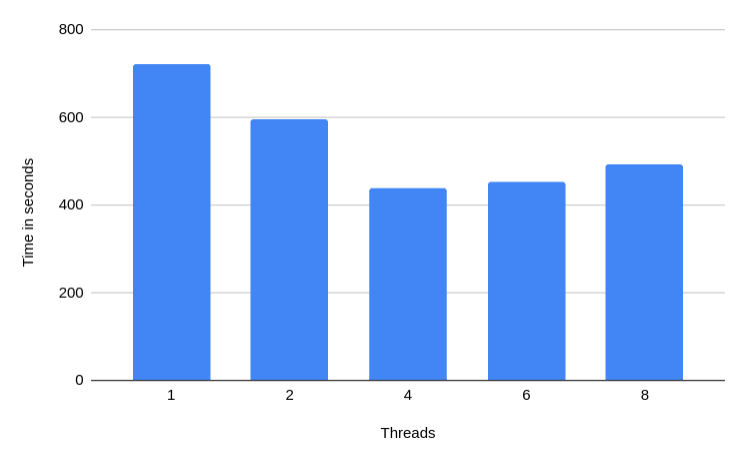
\includegraphics[width=13cm]{figures/threads-table.png}
     \caption{Comparing threads performance.}
     \label{fig:threads-table}
\end{figure}


Another vital step in evaluating the effectiveness of multithreading is examining the distribution of shared links among threads. This is crucial to prevent one thread from overburdening while others remain idle, which would be inefficient, especially when using cloud services like AWS, where resources come at a cost. We'll perform this evaluation using the same configurations from Table \ref{table:crawler_test_config_depth_10}, employing four threads.

Figure \ref{fig:threads-share} displays the results of four runs, with each run showcasing a distinct distribution of crawled links among threads. While the ideal scenario would involve each thread handling 25\% of the discovered links, the averages in the columns reveal variations. Thread $4$ crawls more than 25\%, while Thread $1$ crawls less, which is normal due to considerations like communication overhead and thread-specific conditions. Additionally, threads won't split links if their queue contains fewer than five links, further affecting equal distribution.

\begin{figure}[H]	
     \centering
     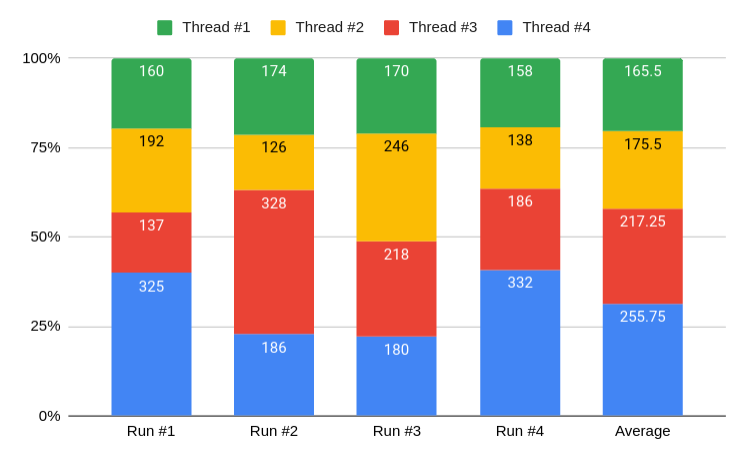
\includegraphics[width=13cm]{figures/threads_share.png}
     \caption{Threads documents distribution.}
     \label{fig:threads-share}
\end{figure}


In order to assess the versatility of the web crawler and its adaptability to various usage scenarios, we will test three additional websites. The initial test case involves crawling a university ranking website to retrieve comprehensive information about all the universities listed, including their titles, respective countries, and current world rankings. The configuration parameters used for crawling this university-ranking website are detailed in Table \ref{table:crawler_conf_uni}.
To accommodate the structure of the website, where each page displays a table containing 25 universities, the "Allow Multi Element" flag is set to True. Considering the pagination feature on the website, which goes up to page 94, we have set the "Max Pages" parameter to 100, as it is unlikely that there will be more than 100 pages to crawl. Since we aim to extract three distinct pieces of information from the table, namely each university's Title, Location, and Ranking, we require three separate inspectors.
Given that each page comprises 25 universities, and there are 94 pages in total, we estimate a maximum of 2,350 documents to be collected during the crawling process.


\begin{table}[ht] 
{\footnotesize
\begin{tabular}{ |p{2.5cm}||p{10.3cm}|  }
 \hline \hline
\textbf{Seed URL} & \href{https://www.timeshighereducation.com/world-university-rankings/2023/world-ranking}{https://www.timeshighereducation.com/world-university-rankings/2023/world-ranking}\T\B 
\\ 
\hline
\textbf{Allow Multi Elements} & True \T\B 
\\ 
\hline
\textbf{Max Pages} & 100\T\B 
\\ 
\hline
\textbf{Threads} & 1\T\B 
\\ 
\hline
\textbf{Max Depth} & 100\T\B 
\\ 
\hline
\textbf{Pagination} & //*[contains(@class, 'pagination')]\T\B 
\\ 
\hline
\textbf{Actions} & None\T\B 
\\ 
\hline
\textbf{Inspectors} & //*[contains(@class, 'ranking-institution-title')] \newline //*[contains(concat(' ', normalize-space(@class), ' '), ' location ')] \newline //*[contains(@class, 'rank') and contains(@class, 'sorting\_1') and contains(@class, 'sorting\_2')]
\T\B 
\\ 
\hline
\textbf{Max Docs} & 2350\T\B 
\\ 
\hline \hline
    \end{tabular}
}
  \captionsetup{justification=centering,margin=2cm}
  \caption{Crawler configuration}
  \label{table:crawler_conf_uni}
\end{table}

The collected and visited links are accurate and match the expected count of 94. The fact that there are zero already visited links indicates that no duplicate URLs have been encountered. The total time spent during this process is approximately 8 minutes, which is significantly shorter compared to a similar test conducted using ParseHub, which took 20 minutes to complete all 94 pages.
Interestingly, even though the crawler successfully parsed and collected the results correctly, it consistently received a 403\footnote{The HTTP 403 Forbidden status code signifies that the server comprehends the request but declines to grant authorization for it.} status code in response to all HTTP requests instead of the expected 200. This issue may be attributed to the website's use of Cloudflare service, as suggested by the information available at ScrapeOps\footnote{\url{https://scrapeops.io/web-scraping-playbook/403-forbidden-error-web-scraping/}} .
In this particular use case, the number of collected documents representing universities in the table matches the total results displayed in the page pagination, totalling 2345. It is worth noting that the website also deploys a Robots.txt file, which the crawler successfully detected and used.

\begin{table}[ht] 
{\footnotesize
\begin{tabular}{ |p{2.5cm}||p{10.3cm}|  }
 \hline \hline
\textbf{Links} & 
\begin{tabular}{c|c|c|c|c}
       Collected   & Visited Correctly & Already Visited & Cross Site &  Excluded\T\B \\\hline
       94/94 & 94 & 0 & 0 & 0
\end{tabular}
\\ 
\hline
\textbf{Time} &
\begin{tabular}{ |p{3cm}||p{3cm}||p{3cm}|  }
       Tot. Spent & Avg. Processing & Avg. Page Rendering \T\B \\\hline
       351.66 s & 2.57 s & 1.020 s 
\end{tabular}
\\
\hline
\textbf{Status Codes} &  403: 94\T\B 
\\ 
\hline
\textbf{Docs \& Content} & 
\begin{tabular}{c|c|c|c}
       Tot. Docs   & Duplicated Content & Avg. Docs Per Page & Avg. Page Size\T\B \\\hline
       2345 & 0 & 25 & 0.2227
\end{tabular}
\\ 
\hline
\textbf{Robots.txt Exists} & True\T\B 
\\ 
\hline
\textbf{Tot. Errors} & 0\T\B 
\\ 
\hline \hline
    \end{tabular}
}
  \captionsetup{justification=centering,margin=2cm}
  \caption{Crawler configuration}
  \label{table:crawler_result_uni}
\end{table}


The following use case involves extracting a specific category of products from an e-commerce website. In this scenario, we will gather various types of data, including text and images. You can find the crawler configurations for this task in Table \ref{table:crawler_conf_douglas}, designed to scrape a particular product category.
Given that the Seed URL link's pagination indicates the presence of 7 pages, we can configure the Max Pages and Max Docs parameters to be 10. We can employ multithreading to increase performance by setting the number of threads to 4. Douglas employs lazy loading for image loading, which, in turn, causes the crawler to fetch only 30 out of the available 48 products on the page. To address this issue, we can utilize the actions tab to introduce a scrolling action, repeating it ten times until we reach the bottom of the page.
The ability to configure automated actions depends on the website's functionality. For instance, if the website experiences prolonged loading times, we can include a waiting action to account for the estimated waiting time. If the website necessitates a clicking action to reveal more information, the click action can be utilized for that purpose. The inspectors in this context encompass four fields: brand, title, price, and product images.


\begin{table}[ht] 
{\footnotesize
\begin{tabular}{ |p{2.5cm}||p{10.3cm}|  }
 \hline \hline
\textbf{Seed URL} & \href{https://www.douglas.de/de/c/parfum/damenduefte/duftsets/010111}{https://www.douglas.de/de/c/parfum/damenduefte/duftsets/010111}\T\B 
\\ 
\hline
\textbf{Allow Multi Elements} & True \T\B 
\\ 
\hline
\textbf{Max Pages} & 10\T\B 
\\ 
\hline
\textbf{Threads} & 4\T\B 
\\ 
\hline
\textbf{Max Depth} & 10\T\B 
\\ 
\hline
\textbf{Pagination} & //*[contains(@class, 'pagination')]\T\B 
\\ 
\hline
\textbf{Actions} & Scolling down 10 times\T\B 
\\ 
\hline
\textbf{Inspectors} & //*[contains(@class, 'top-brand')]\T\B  \newline
//a[contains(@class, 'product-tile\_\_main-link')]/div[1]/div/img \newline
//*[contains(@class, 'text')][contains(@class, 'name')] \newline
//div[contains(concat(' ', normalize-space(@class), ' '), ' price-row ')]\B  
\\ 
\hline
\textbf{Max Docs} & 1000\T\B 
\\ 
\hline \hline
    \end{tabular}
}
  \captionsetup{justification=centering,margin=2cm}
  \caption{Crawler configuration}
  \label{table:crawler_conf_douglas}
\end{table}

Table \ref{table:crawler_result_douglas} displays the outcomes obtained following the execution of the Douglas crawler. The "Collected" and "Visited" links align with the expected numbers within the targeted pagination. The estimated time taken for this operation is approximately 6.7 minutes. Notably, the "Average processing time" is more than double the time reported in the uni-ranking results in Table \ref{table:crawler_result_uni}. The primary reason for this extended processing time is the inclusion of additional scrolling-down actions.

It is noteworthy to consider an alternative approach: instead of scrolling down ten times to reach the page's end for image loading, why not employ a "scroll to the end of the page" event? This approach was tested on the Douglas website but proved ineffective. The reason is that specific frontend frameworks only load content when it is within the browser's view. Additionally, some websites, such as Facebook, initially display a limited number of posts on a user's home page, progressively loading more as the user scrolls down. In such cases, a single "jump to the end of the page" action will not suffice, as multiple scrolling-down actions are required.

The total count of collected documents indicates that 245 products were downloaded, which appears to be less than anticipated. Given that there are seven pages, with the first page containing 48 products, the theoretical result should be around 336 products. Further investigation revealed that only some pages contain exactly 48 products; some have more, while others have fewer.

It is important to note that, despite employing the robots.txt file for politeness and ensuring a relatively low crawler request rate (calculated as the number of threads divided by the Average Page Rendering, yielding 1.516 requests per second, which is relatively low and unlikely to overload the server), the IP address was eventually banned, and access to the site was blocked after several attempts. This highlights that each website may have its own unique security implementation based on its firewall\footnote{A firewall is a network security tool that filters and controls network traffic to safeguard against unauthorized access and cyber threats, serving as a barrier between trusted internal networks and untrusted external networks, such as the Internet.} rules and the reverse proxy\footnote{A reverse proxy is a server or software component that sits between client devices and a web server, forwarding client requests to the appropriate server and often providing additional functionalities like load balancing, caching, and security protection.} it uses.

Additionally, it's worth mentioning that the Douglas crawler was used without issue for three months, but a ban was encountered recently. This underscores that websites can adapt and modify their security measures over time.

\begin{table}[ht] 
{\footnotesize
\begin{tabular}{ |p{2.5cm}||p{10.3cm}|  }
 \hline \hline
\textbf{Links} & 
\begin{tabular}{c|c|c|c|c}
       Collected   & Visited Correctly & Already Visited & Cross Site &  Excluded\T\B \\\hline
       7/7 & 7 & 0 & 0 & 0
\end{tabular}
\\ 
\hline
\textbf{Time} &
\begin{tabular}{ |p{3cm}||p{3cm}||p{3cm}|  }
       Tot. Spent & Avg. Processing & Avg. Page Rendering \T\B \\\hline
       395.209 s & 7.87 s & 2.638 s 
\end{tabular}
\\
\hline
\textbf{Status Codes} & 200: 7\T\B 
\\ 
\hline
\textbf{Docs \& Content} & 
\begin{tabular}{c|c|c|c}
       Tot. Docs   & Duplicated Content & Avg. Docs Per Page & Avg. Page Size\T\B \\\hline
       245 & 0 & 49 & 1.509
\end{tabular}
\\ 
\hline
\textbf{Robots.txt Exists} & True\T\B 
\\ 
\hline
\textbf{Tot. Errors} & 0\T\B 
\\ 
\hline \hline
    \end{tabular}
}
  \captionsetup{justification=centering,margin=2cm}
  \caption{Crawler results}
  \label{table:crawler_result_douglas}
\end{table}


Parshub encountered a crash while running Douglas's project, resulting in the error message: "Segmentation fault (core dumped)." Although this made it challenging to compare performance, it shed light on Parsehub's stability issues, as Parsehub frequently struggles to handle websites without crashing.

Another use case involved crawling Stackoverflow questions, focusing solely on the "python" tag in the seed URL to retrieve Python-related questions. The configured inspectors collected question titles, descriptions, and vote counts. Initially, running the crawler with four threads led to a website ban after only ten pages were crawled. To resolve this, I reduced the thread count to one, reducing the number of requests and resolving the issue.


\begin{table}[ht] 
{\footnotesize
\begin{tabular}{ |p{2.5cm}||p{10.3cm}|  }
 \hline \hline
\textbf{Seed URL} & \href{https://stackoverflow.com/questions/tagged/python}{https://stackoverflow.com/questions/tagged/python}\T\B 
\\ 
\hline
\textbf{Allow Multi Elements} & True \T\B 
\\ 
\hline
\textbf{Max Pages} & 100\T\B 
\\ 
\hline
\textbf{Threads} & 1\T\B 
\\ 
\hline
\textbf{Max Depth} & 100\T\B 
\\ 
\hline
\textbf{Pagination} & //*[contains(@class, 's-pagination')]\T\B 
\\ 
\hline
\textbf{Actions} & None\T\B 
\\ 
\hline
\textbf{Inspectors} & //*[contains(@class, 's-post-summary--content-title')]\T\B  \newline
//*[contains(@class, 's-post-summary--content-excerpt')]	
 \newline
//*[contains(@class, 's-post-summary--stats-item\_\_emphasized')]	
\\ 
\hline
\textbf{Max Docs} & 1000\T\B 
\\ 
\hline \hline
    \end{tabular}
}
  \captionsetup{justification=centering,margin=2cm}
  \caption{Crawler configuration}
  \label{table:crawler_conf_stack}
\end{table}


Table \ref{table:crawler_result_stack} presents the crawler's results after this thread adjustment. Notably, the collected links exceeded those displayed in the pagination, indicating an issue with the pagination selector "s-pagination" collecting additional links. The number of visited pages reached 100, the configured limit, as intended, preventing the crawler from continuing to crawl all 27,200 found links. Many cross-site and excluded links signalled that the crawler had lost track and was collecting incorrect links. While 885 documents were collected correctly, there was no guarantee that they were all related to the chosen "Python" topic. Fortunately, termination conditions like Max Pages, Max Docs, and Max Depth were in place to conserve resources.

To troubleshoot the crawler, I enabled the 'Show Browser' option and reran it. This allowed for easier visualization of the crawler's behaviour and the links it was crawling. It revealed that the crawler was indeed lost and opening the wrong links. Despite the correct seed URL and pagination, the pagination selector 's-pagination' was missing from the configuration. This issue demonstrates how easy it is to debug and identify problems when a crawler loses its way, highlighting the crawler's politeness and stability.


\begin{table}[ht] 
{\footnotesize
\begin{tabular}{ |p{2.5cm}||p{10.3cm}|  }
 \hline \hline
\textbf{Links} & 
\begin{tabular}{c|c|c|c|c}
       Collected   & Visited Correctly & Already Visited & Cross Site &  Excluded\T\B \\\hline
       27200 & 100 & 0 & 460 & 666
\end{tabular}
\\ 
\hline
\textbf{Time} &
\begin{tabular}{ |p{3cm}||p{3cm}||p{3cm}|  }
       Tot. Spent & Avg. Processing & Avg. Page Rendering \T\B \\\hline
       588.505 s & 6.38 s & 0.561 s 
\end{tabular}
\\
\hline
\textbf{Status Codes} & 200: 99, 404:1 \T\B 
\\ 
\hline
\textbf{Docs \& Content} & 
\begin{tabular}{c|c|c|c}
       Tot. Docs   & Duplicated Content & Avg. Docs Per Page & Avg. Page Size\T\B \\\hline
       885 & 241 & 14 & 0.155
\end{tabular}
\\ 
\hline
\textbf{Robots.txt Exists} & True\T\B 
\\ 
\hline
\textbf{Tot. Errors} & 0\T\B 
\\ 
\hline \hline
    \end{tabular}
}
  \captionsetup{justification=centering,margin=2cm}
  \caption{Crawler results}
  \label{table:crawler_result_stack}
\end{table}

After fixing the second issue and rerunning the crawler, it operated correctly and yielded results in Table \ref{table:crawler_result_stack_2}. Notably, cross-site and excluded links were reduced to zero, a positive sign. Additionally, the number of collected links was lower than in the first attempt, totalling 900, with nine links collected per page. Interestingly, there were a significant number of 404 and 429 status codes. To address this, it could be beneficial to include a wait action between requests to mitigate the 429 errors.

When the same test was conducted using ParseHub, it took 20 minutes to complete, which was slower than the crawler's 6-minute runtime. It is worth noting that the two issues encountered during crawling were not experienced with ParseHub. This is because ParseHub's request rate is slower, reducing the risk of being banned. This is achieved by reducing the number of threads and can be further improved by adding wait actions. The second issue, concerning incorrect selectors, is where ParseHub shines as it offers an easy autodetect feature, simplifying selector selection with a simple click instead of manual XPATH insertion as required in the current crawler implementation.

\begin{table}[ht] 
{\footnotesize
\begin{tabular}{ |p{2.5cm}||p{10.3cm}|  }
 \hline \hline
\textbf{Links} & 
\begin{tabular}{c|c|c|c|c}
       Collected   & Visited Correctly & Already Visited & Cross Site &  Excluded\T\B \\\hline
       900 & 100 & 0 & 0 & 0
\end{tabular}
\\ 
\hline
\textbf{Time} &
\begin{tabular}{ |p{3cm}||p{3cm}||p{3cm}|  }
       Tot. Spent & Avg. Processing & Avg. Page Rendering \T\B \\\hline
       354.734 s & 2.66 s & 0.155 s 
\end{tabular}
\\
\hline
\textbf{Status Codes} & 200: 54, 404:21, 429: 25 \T\B 
\\ 
\hline
\textbf{Docs \& Content} & 
\begin{tabular}{c|c|c|c}
       Tot. Docs   & Duplicated Content & Avg. Docs Per Page & Avg. Page Size\T\B \\\hline
       2750 & 0 & 50 & 0.155
\end{tabular}
\\ 
\hline
\textbf{Robots.txt Exists} & True\T\B 
\\ 
\hline
\textbf{Tot. Errors} & 0\T\B 
\\ 
\hline \hline
    \end{tabular}
}
  \captionsetup{justification=centering,margin=2cm}
  \caption{Crawler results}
  \label{table:crawler_result_stack_2}
\end{table}

\section{Indexer}  

Following the initial crawling phase, the next step involves indexing, which requires a dedicated section for evaluation. To perform a thorough assessment of indexing, we will utilize a real-world dataset obtained through one of the crawlers employed during the evaluation process. We selected the Stack Overflow dataset presented in Table \ref{table:crawler_conf_stack} out of the three available use cases. The primary rationale for this choice is its larger size compared to the others, along with the presence of descriptions that can be employed for index evaluation. It is important to note that the crawler was rerun to gather additional Stack Overflow posts.

\subsection{Datasets}


\begin{table}[ht] 
{\footnotesize
\begin{tabular}{ |p{2.5cm}||p{10.3cm}|  }
 \hline \hline
\textbf{File Size} & 1.4MB \T\B 
\\ 
\hline
\textbf{Entries Count} & 2415\T\B 
\\ 
\hline
\textbf{Words Count} & 108122\T\B 
\\ 
\hline
\textbf{Fields} & Title, Summary, Votes\T\B 
\\ 
\hline \hline
    \end{tabular}
}
  \captionsetup{justification=centering,margin=2cm}
  \caption{Stack Overflow posts dataset}
    \label{table:indexer_dataset}
\end{table}

\subsection{Metrics}
We assess precision at a given value k (P@k), calculate the average precision (AP), and compute the normalized discounted cumulative gain at a specific position k (nDCG@k).

\subsection*{Precision at k (P@k)}
P@k represents the proportion of valid predictions within the system's top k predictions. We define $Q_{valid}$ as the collection of valid predictions for a question prefix q, as specified in the ground truth. Additionally, we denote $Q^k_{result}$ as the set of the system's top k completion predictions for a given question prefix q. The calculation for P@k is as follows:

\begin{equation}
P@k = \frac{|Q_{valid} \cap Q^k_{result}|}{k}
\label{eq:depth}
\end{equation}

We will compute the precision at 5 (p@5) for all the various indexing configurations.

\subsection*{Average Precision (AP)}
Consider $R_1$ through $R_k $ as the ordered list of positions where relevant documents are located within the result list of a specific query. In this context, Average Precision (AP) is computed as the mean of the k Precision at $R_i$ ($P@R_i$) values. AP is computed as:

\begin{equation}
AP = \frac{\sum_{i=1}^{n} P@r_i}{n}
\label{eq:depth}
\end{equation}

For the predictions from $Q_{valid}$ that are absent in $Q_{result}$, we assign a Precision at position $r_i $ (P@ri) value of 0. We then calculate the average precision by averaging these values across all question prefixes in the ground truth.

\subsection*{Mean Precisions (MP@k, MP@R, MAP)}
Having a benchmark containing multiple queries and their corresponding ground truth data, we can assess the system's performance by calculating the average value of a specific metric across all the queries.

MP@k represents the mean precision at k values across all queries, MP@R represents the mean precisionat R values across all queries, and MAP signifies the mean average precision values across all queries.

\subsection{Experiments}
 
 To assess the performance of our indexing, we will employ the Stack Overflow dataset listed in Table \ref{table:indexer_dataset}. We will modify the indexing attributes' settings and examine how these changes impact the evaluation metrics.
 
 We will initiate our indexing process using the default settings specified in Table \ref{table:indexer_conf_1}. The Stack Overflow dataset consists of three inspector fields: Title, Summary, and Votes. However, we intend to index only the textual fields, such as Title and Summary, while retaining Votes as they contain numerical data intended solely for ranking purposes. All other configuration parameters are set to their default values. For a clearer understanding of the configuration attributes, please refer to Table \ref{table:indexing-config}, which provides descriptions of each attribute.
 


\begin{table}[ht] 
{\footnotesize
\begin{tabular}{ |p{2.5cm}||p{10.3cm}|  }
 \hline \hline
\textbf{Inspectors} & Title, Summary \T\B 
\\ 
\hline
\textbf{BM25 Parameters} & B=0.75, K=1.75\T\B 
\\ 
\hline
\textbf{Stop Words} & None\T\B 
\\ 
\hline
\textbf{Small Words Threshold} & 2\T\B 
\\ 
\hline
\textbf{Q-gram} & 3\T\B 
\\ 
\hline
\textbf{Boosting Formula} & None\T\B 
\\ 
\hline
\textbf{Result} & 
\begin{tabular}{ |p{2cm}||p{2cm}||p{2cm}||p{2cm}|  }
       \textbf{MP@5} & \textbf{MP@R} & \textbf{MAP} & \textbf{Time(s)}\T\B \\\hline
       0.73 & 0.72 & 0.87 & 0.31
\end{tabular}
\\
\hline \hline
    \end{tabular}
}
  \captionsetup{justification=centering,margin=2cm}
  \caption{Stack Overflow indexing configuration, test the default settings without any changes.}
      \label{table:indexer_conf_1}
\end{table}

Upon initiating the indexing process for the first time, without the availability of any caching, it may take up to two minutes to complete. This indexing procedure consists of two distinct stages: the first involves the creation of a dictionary, which aids in providing suggestions in the dropdown menu to help users locate the appropriate queries. Creating this dictionary is the longer of the two stages, typically taking around 1.8 minutes, while the indexing phase takes approximately seven seconds. The primary disparity between these stages lies in the size of the entities involved; the dictionary comprises 2.6 million entities, whereas the Stack Overflow entities used for indexing consist of only two thousand entities. It is worth noting that the overall duration of the indexing process is highly contingent on the size of the file being indexed and, in this case, the volume of documents crawled by the web crawler. Following the initial indexing process, the dictionary index will be cached and no longer require further indexing.

Even though the search results return 25 documents, we will set the value of k for the P@k metric to 5. This choice is based on the everyday user preference for focusing on the top results in a search list. The overall metrics are presented in Table \ref{table:indexer_conf_1}. While these results indicate reasonable accuracy, it is essential to acknowledge that assessing relevance can be subjective, as it varies among users. For instance, Google's ranking system considers factors like user location, link authenticity, and text matching, leading to potentially inconsistent results for the same query across different users.
Furthermore, aiming for an extremely high level of accuracy can lead to model overfitting\footnote{Overfitting in data science happens when a model fits its training data too closely. This leads to poor performance when dealing with new, unseen data.}, causing it to struggle with generalization. While it may achieve a high precision score with benchmark data, it may need to improve when faced with new, unseen queries. This is because all the model's parameters have been fine-tuned to fit the benchmark datasets perfectly. Therefore, balancing achieving a reasonable precision score and ensuring that the model performs well on new, previously unseen datasets is crucial. Therefore, achieving perfect accuracy scores in evaluations is challenging and involves a trade-off. The Precision@K metric is significantly affected by the selection of both the value of K and the relevance threshold. Different choices for K and the threshold can result in varying Precision@K scores for the same model. As a result, it is essential to carefully and consistently choose these parameters when comparing different models.

\begin{table}[ht] 
{\footnotesize
\begin{tabular}{ |p{2.5cm}||p{10.3cm}|  }
 \hline \hline
\textbf{Inspectors} & Title, Summary \T\B 
\\ 
\hline
\textbf{BM25 Parameters} & B=0.1, K=0.81\T\B 
\\ 
\hline
\textbf{Stop Words} & None\T\B 
\\ 
\hline
\textbf{Small Words Threshold} & 2\T\B 
\\ 
\hline
\textbf{Q-gram} & 3\T\B 
\\ 
\hline
\textbf{Boosting Formula} & None\T\B 
\\ 
\hline
\textbf{Result} & 
\begin{tabular}{ |p{2cm}||p{2cm}||p{2cm}||p{2cm}|  }
       \textbf{MP@5} & \textbf{MP@R} & \textbf{MAP} & \textbf{Time(s)}\T\B \\\hline
       0.8 & 0.84 & 0.89 & 0.31
\end{tabular}
\\
\hline \hline
    \end{tabular}
}
  \captionsetup{justification=centering,margin=2cm}
  \caption{Stack Overflow indexing configuration}
  \label{table:indexer_conf_2}
\end{table}

The initial parameters to adjust are b and k. Table \ref{table:indexer_conf_2} displays the configuration of the Stack Overflow indexer, with modifications made to the default b and k values. These values have increased. The key takeaway is that modifying the attributes available in the indexing user interface can enhance or diminish accuracy, providing users with a convenient way to fine-tune their model.

\begin{table}[ht] 
{\footnotesize
\begin{tabular}{ |p{2.5cm}||p{10.3cm}|  }
 \hline \hline
\textbf{Inspectors} & Title, Summary \T\B 
\\ 
\hline
\textbf{BM25 Parameters} & B=0.1, K=0.81\T\B 
\\ 
\hline
\textbf{Stop Words} & how, to, by, with, in, not, does\T\B 
\\ 
\hline
\textbf{Small Words Threshold} & 2\T\B 
\\ 
\hline
\textbf{Q-gram} & 3\T\B 
\\ 
\hline
\textbf{Boosting Formula} & None\T\B 
\\ 
\hline
\textbf{Result} & 
\begin{tabular}{ |p{2cm}||p{2cm}||p{2cm}||p{2cm}|  }
       \textbf{MP@5} & \textbf{MP@R} & \textbf{MAP} & \textbf{Time(s)}\T\B \\\hline
       0.66 & 0.624 & 0.76 & 0.31
\end{tabular}
\\
\hline \hline
    \end{tabular}
}
  \captionsetup{justification=centering,margin=2cm}
  \caption{Stack Overflow indexing configuration}
    \label{table:indexer_conf_3}
\end{table}


Let us retain the modified b and k parameters instead of using the default values, as they produce improved results. The following attribute we consider for indexing includes stop words and examining their impact on accuracy. Initially, the intuition is to remove common words such as "how," "to," "by," "with," "in," "not," and "does" from the benchmark queries since they may seem insignificant and lack essential information. Surprisingly, though, removing these words leads to a reduction in accuracy as illustraded in Table \ref{table:indexer_conf_3}.

This could be attributed to the Stack Overflow dataset not being exceptionally large, and the assumption that these words are common in the English language may not hold for some queries in the small Stack Overflow dataset. Furthermore, stop words are not just about eliminating common words; they can also be used to consistently disregard words that typically provide no meaningful information in a query. For example, in the current Stack Overflow dataset, which encompasses all posts related to Python, including the term "python" in the query should have no impact, as all the posts are Python-related, even if they do not explicitly mention the word "python" but discuss Python libraries, for instance.

It is important to note that stop words containing two characters or fewer have no impact in this context and can be safely eliminated. The rationale is that they should already be filtered out due to the Small Words Threshold being set to two.


\begin{table}[ht] 
{\footnotesize
\begin{tabular}{ |p{2.5cm}||p{10.3cm}|  }
 \hline \hline
\textbf{Inspectors} & Title, Summary \T\B 
\\ 
\hline
\textbf{BM25 Parameters} & B=0.1, K=0.81\T\B 
\\ 
\hline
\textbf{Stop Words} & None\T\B 
\\ 
\hline
\textbf{Small Words Threshold} & 0\T\B 
\\ 
\hline
\textbf{Q-gram} & 3\T\B 
\\ 
\hline
\textbf{Boosting Formula} & None\T\B 
\\ 
\hline
\textbf{Result} & 
\begin{tabular}{ |p{2cm}||p{2cm}||p{2cm}||p{2cm}|  }
       \textbf{MP@5} & \textbf{MP@R} & \textbf{MAP} & \textbf{Time(s)}\T\B \\\hline
       0.8 & 0.77 & 0.84 & 0.31
\end{tabular}
\\
\hline \hline
    \end{tabular}
}
  \captionsetup{justification=centering,margin=2cm}
  \caption{Stack Overflow indexing configuration}
  \label{table:indexer_conf_4}
\end{table}

In the following evaluation in Table \ref{table:indexer_conf_4}, we adjust the Small Words Threshold to zero, which implies that no words are excluded during the indexing process. While the results remain reasonably good, there has been a decrease in precision. This suggests that in certain cases, increasing the Small Words Threshold and not setting it to zero may be advisable. However, it's essential to exercise caution when eliminating small words, particularly those with one to three characters, depending on the language. Additionally, it's worth noting that some two-character words can be acronyms, such as "OS" (Operating System).

\begin{table}[ht] 
{\footnotesize
\begin{tabular}{ |p{2.5cm}||p{10.3cm}|  }
 \hline \hline
\textbf{Inspectors} & Title, Summary \T\B 
\\ 
\hline
\textbf{BM25 Parameters} & B=0.1, K=0.81\T\B 
\\ 
\hline
\textbf{Stop Words} & None\T\B 
\\ 
\hline
\textbf{Small Words Threshold} & 2\T\B 
\\ 
\hline
\textbf{Q-gram} & 3\T\B 
\\ 
\hline
\textbf{Boosting Formula} & $\frac{votes}{10}$\T\B 
\\ 
\hline
\textbf{Result} & 
\begin{tabular}{ |p{2cm}||p{2cm}||p{2cm}||p{2cm}|  }
       \textbf{MP@5} & \textbf{MP@R} & \textbf{MAP} & \textbf{Time(s)}\T\B \\\hline
       0.53 & 0.62 & 0.63 & 0.31
\end{tabular}
\\
\hline \hline
    \end{tabular}
}
  \captionsetup{justification=centering,margin=2cm}
  \caption{Stack Overflow indexing configuration}
  \label{table:indexer_conf_5}
\end{table}

The final attribute to adjust is the Boosting Formula. The Boosting Formula is an optional field and particularly useful for ranking documents containing a numeric field. Examples of such fields include product prices, product reviews, post likes, post shares, or the order of items in a list, like the example of university rankings.
In the specific context of the Stack Overflow example, each post is associated with an upvote number, which indicates how helpful an answer is. This numeric field can be a valuable indicator of document quality and relevance. The more users find a post helpful, the more valuable it becomes to display it as one of the top results. To assign a higher score to posts with a high number of votes, we can employ the Boosting Formula. One practical choice is to use the logarithm of the votes. However, since votes can be zero or even negative, more suitable options may exist. We will utilize the formula shown in \ref{table:indexer_conf_5} for this straightforward use case.


\section{User Experience} 

Throughout this project, I had the opportunity to work with ParseHub software. While this experience does not make me an expert, I did gain practical knowledge in using ParseHub for various aspects of web crawling, which proved beneficial for the thesis. There are notable advantages and disadvantages when comparing ParseHub with the current implementation used in the thesis.

One of the standout features of ParseHub is its automatic detection of document fields, achieved by clicking. In contrast, my implementation requires manual input of HTML element XPATH to obtain this information. Creating the crawlers manually in my implementation often took more than ten minutes, whereas ParseHub accomplished the same results in half the time. Another advantage of ParseHub is its project-based approach to crawling, as opposed to my implementation's list of crawlers. Starting a crawler in ParseHub can be done by providing only the Seed URL without further options, simplifying the process. However, it is essential to note that this feature can be easily extended and is a manageable hurdle.

In terms of performance, the current implementation excels, as demonstrated in the evaluation tables. Additionally, the current implementation allows for the addition of more threads and nodes to enhance performance, a flexibility not available in ParseHub. Furthermore, the current implementation has proven resilient in handling various edge cases, whereas ParseHub struggled to manage these scenarios effectively. The adaptability and configuration options offered by the current implementation make it well-suited for various websites and scenarios.

The user interface employed in ParseHub needs to be updated; it lacks responsiveness and features a font that is challenging to read. However, the most frustrating aspect is the frequent occurrence of the browser unexpectedly crashing and shutting down without apparent cause. In contrast, utilizing a frontend framework like Angular with PrimeNG significantly improved the current implementation, making it responsive and delivering a seamless user experience.

One notable drawback of ParseHub is its need for indexing capabilities. When crawling a large dataset, having an indexed version of the data becomes crucial, mainly if the dataset is intended to be served as an API, for example.
    \chapter{Conclusions and Future Work}\label{chap:conclusion}

Within this chapter, we address the questions initially introduced at the opening of the thesis (Section \ref{sec:contribution}), conclude our experiments, and open the door for additional research to enhance the solution and explore areas that have not been previously examined.
\section{Conclusions}

It is crucial to remember the primary questions and contributions intended to be accomplished by this thesis and whether we have successfully addressed them or if they remain abstract. In the following list, we iterate through the contributions mentioned in Section \ref{sec:contribution}  and discuss our final findings.

\begin{itemize}
  \item \textit{What are the challenges and bottlenecks to creating a scalable, configurable search engine?}
Two primary bottlenecks restrict the crawler's performance. The first is the loading time, or the time it takes to render a page, which varies for each page and ultimately affects the rate at which the crawler can make requests. The second challenge is that websites can block the crawler if the request rate increases, which is also contingent on the configurations of the websites' firewalls.

\item \textit{Can we outperform a similar tool like ParseHub?}
ParseHub demonstrated an advantage with its smoother workflow and improved automated field selection. Nonetheless, Scriburg surpassed ParseHub in terms of performance and overall robustness.

\item \textit{How does changing the configurations provided by the user interface affect the results in the crawling and indexing accuracy?} The user interface offers forms, including optional and advanced crawling and indexing options. The used options deliver a helpful and adaptable user experience. Even users with limited programming experience can easily configure and execute straightforward crawling and indexing tasks by relying on the default values provided.

    \item \textit{Can we create a decent User Interface UI that intuitively allows users to crawl and index targeted websites from the internet?} Yes, we did. However, manually adding and removing inspectors was time-consuming and should be refined.
    
\item \textit{How well do crawlers react to different websites with different DOM structures?} While the internet hosts millions of websites, making it impossible to ensure coverage for all possible use cases, we have evaluated many websites and effectively managed their diverse implementations.

    \item \textit{Can we integrate the indexing and crawling processes in the same tool?} It was possible to provide a user-friendly interface that combines both functionalities.
    
    \item \textit{Can we find meaningful evaluation metrics for the implemented search engine?} We have discovered that evaluating crawling can pose challenges, but certain aspects can be addressed to provide insights into the crawler's performance.
    
\end{itemize}

\section{Future Work}
While evaluating \textbf{Scriburg}, the most wanted feature was to automate the inspector's selections. The solution should be similar to what \textbf{ParseHub} is implementing. The user should be faced with a live session where they can click on any title or price they want to collect simply by clicking. However, This feature is not easy to implement and can take up to \textbf{three months} to perfect. 

Adding \textbf{IP Rotation} is highly recommended because although the crawling rate was not high in the evaluation, the crawler got banned twice from different websites. Implementing IP Rotation is relatively easy. Some services provide free proxy list API\footnote{SSL Proxies: \url{https://www.sslproxies.org/}} to be used to make proxied requests. One can add each proxy bypassing the flag \texttt{proxy-server} in Selenium. This feature can take up to \textbf{three days} to implement and test.

Adding a \textbf{Steps}\footnote{PrimeNG Steps: \url{https://primeng.org/steps/personal}} component can allow the users to crawl and index step by step. For example, the first step is to create a project name like Stack Overflow. This name will be used for all templates, runners, crawlers, and indexers instead of entering the name in each form. The steps will make running a crawler intuitive and reduce user confusion. Using the \textbf{Steps} component from \textbf{PrimeNg} will take \textbf{two weeks} to implement and add this functionality. This feature can solve the issue by making the user interface more intuitive and easily used.

Early stopping the crawlers once they are inefficient helps save resources. This can be due to an internet connection; the website is down, the crawler needs to be better configured, and more issues can make crawling inefficient. Although we are serving valuable information to help monitor the crawling process, for non-technical users, it can be hard to understand what the HTTP status codes stand for. To fix this, we can set up some rules to convert errors into valuable messages that users can understand. This feature can take between \textbf{two weeks} to \textbf{one month} to implement.

Leveraging the \texttt{robots.txt} file to direct web crawlers can be effective, but there is a need for further research into establishing a robust protocol for crawler behavior. For instance, it proves beneficial for crawlers to gain insights into website characteristics, such as estimating the number of links, products, or items present. This information helps users in determining the appropriate scaling of their crawlers. Additionally, the file can specify the maximum allowable requests per second to prevent potential denial-of-service (DoS) issues. It could also contain preferences regarding crawl timings, such as restricting activity to nighttime.

    \chapter{Acknowledgments}

First and foremost, I would like to thank:
\begin{itemize}
    \setlength{\itemsep}{0pt} % Reduce spacing between items
    \setlength{\parskip}{0pt} % Reduce spacing between paragraphs within items
    \setlength{\parsep}{0pt} % Reduce spacing between paragraphs within items
    \setlength{\topsep}{0pt} % Reduce spacing before and after the list

    \item My parents for supporting me during the master's program.
    \item My wife for her love and support.
    \item Prof. Dr. Hannah Bast for accepting my topic and for her supervision.
    \item My advisor Natalie Prange for her competent opinions and suggestions.
\end{itemize}

    % bibliography is not in the table of contents per default, add it manually
    \addcontentsline{toc}{chapter}{Bibliography}
    \bibliographystyle{apalike}
    \bibliography{bib/topic1,bib/topic2}
    \newpage
    \thispagestyle{empty}
    \mbox{}
    

\end{document}
